% allgem. Dokumentenformat
\documentclass[a4paper,12pt,headsepline]{scrartcl}
%Variablen welche innerhalb der gesamten Arbeit zur Verfügung stehen sollen
\newcommand{\titleDocument}{Bachelorarbeit}
\newcommand{\subjectDocument}{im Studiengang Wirtschaftsinformatik}

% Grafiken aus PNG Dateien einbinden
\usepackage{graphicx}

% Deutsche Sonderzeichen benutzen 
\usepackage{ngerman}

% deutsche Silbentrennung
\usepackage[ngerman]{babel}

% Eurozeichen einbinden
\usepackage[right]{eurosym}

% Umlaute unter UTF8 nutzen
\usepackage[utf8]{inputenc}

% Zeichenencoding
\usepackage[T1]{fontenc}
\usepackage{lmodern}
\usepackage{fix-cm}

% floatende Bilder ermöglichen
%\usepackage{floatflt}

% mehrseitige Tabellen ermöglichen
\usepackage{longtable}

% Unterstützung für Schriftarten
\usepackage{helvet}
\renewcommand{\familydefault}{\sfdefault}

% Packet für Seitenrandabständex und Einstellung für Seitenränder
\usepackage{geometry}
\geometry{left=3.5cm, right=2cm, top=2.5cm, bottom=2cm}

% Paket für Boxen im Text
\usepackage{fancybox}

% bricht lange URLs "schoen" um
\usepackage[hyphens,obeyspaces,spaces]{url}

% Paket für Textfarben
\usepackage{color}
    \definecolor{lightgray}{rgb}{0.95, 0.95, 0.95}
    \definecolor{darkgray}{rgb}{0.4, 0.4, 0.4}
    \definecolor{purple}{rgb}{0.65, 0.12, 0.82}
    \definecolor{ocherCode}{rgb}{1, 0.5, 0} % #FF7F00 -> rgb(239, 169, 0)
    \definecolor{blueCode}{rgb}{0, 0, 0.93} % #0000EE -> rgb(0, 0, 238)
    \definecolor{greenCode}{rgb}{0, 0.6, 0} % #009900 -> rgb(0, 153, 0)
    
    \definecolor{editorGray}{rgb}{0.95, 0.95, 0.95}
    \definecolor{editorOcher}{rgb}{1, 0.5, 0} % #FF7F00 -> rgb(239, 169, 0)
    \definecolor{editorGreen}{rgb}{0, 0.5, 0} % #007C00 -> rgb(0, 124, 0) 

% Mathematische Symbole importieren
\usepackage{amssymb}

% Auflistungen
\usepackage{paralist}

% erzeugt Inhaltsverzeichnis mit Querverweisen zu den Kapiteln (PDF Version)
\usepackage[bookmarksnumbered,pdftitle={\titleDocument},hyperfootnotes=false]{hyperref} 
%\hypersetup{colorlinks, citecolor=red, linkcolor=blue, urlcolor=black}
\hypersetup{colorlinks, citecolor=black, linkcolor= black, urlcolor=black}

% neue Kopfzeilen mit fancypaket
\usepackage{fancyhdr} %Paket laden
\pagestyle{fancy} %eigener Seitenstil
\fancyhf{} %alle Kopf- und Fußzeilenfelder bereinigen
\fancyhead[L]{\nouppercase{\leftmark}} %Kopfzeile links
\fancyhead[C]{} %zentrierte Kopfzeile
\fancyhead[R]{\thepage} %Kopfzeile rechts
\renewcommand{\headrulewidth}{0.4pt} %obere Trennlinie
%\fancyfoot[C]{\thepage} %Seitennummer
%\renewcommand{\footrulewidth}{0.4pt} %untere Trennlinie

% für Tabellen
\usepackage{array}

% Runde Klammern für Zitate
%\usepackage[numbers,round]{natbib}

% Festlegung Art der Zitierung - Havardmethode: Abkuerzung Autor + Jahr
\bibliographystyle{alphadin}

% Schaltet den zusätzlichen Zwischenraum ab, den LaTeX normalerweise nach einem Satzzeichen einfügt.
\frenchspacing

% Paket für Zeilenabstand
\usepackage{setspace}

% für Bildbezeichner
\usepackage{capt-of}

% für Stichwortverzeichnis
\usepackage{makeidx}

% für Listings
\usepackage{listings}
%\lstset{numbers=left, numberstyle=\tiny, numbersep=5pt, keywordstyle=\color{black}\bfseries, stringstyle=\ttfamily,showstringspaces=false,basicstyle=\footnotesize,captionpos=b}
\lstdefinelanguage{JavaScript}{
      morekeywords={break, case, catch, continue, debugger, default, delete, do, else, false, finally, for, function, if, in, instanceof, new, null, return, switch, this, throw, true, try, typeof, var, void, while, with},
      morecomment=[s]{/*}{*/},
      morecomment=[l]//,
      morestring=[b]",
      morestring=[b]'
    }

\lstdefinelanguage{CSS}{
      keywords={accelerator,azimuth,background,background-attachment,
            background-color,background-image,background-position,
            background-position-x,background-position-y,background-repeat,
            behavior,border,border-bottom,border-bottom-color,
            border-bottom-style,border-bottom-width,border-collapse,
            border-color,border-left,border-left-color,border-left-style,
            border-left-width,border-right,border-right-color,
            border-right-style,border-right-width,border-spacing,
            border-style,border-top,border-top-color,border-top-style,
            border-top-width,border-width,bottom,caption-side,clear,
            clip,color,content,counter-increment,counter-reset,cue,
            cue-after,cue-before,cursor,direction,display,elevation,
            empty-cells,filter,float,font,font-family,font-size,
            font-size-adjust,font-stretch,font-style,font-variant,
            font-weight,height,ime-mode,include-source,
            layer-background-color,layer-background-image,layout-flow,
            layout-grid,layout-grid-char,layout-grid-char-spacing,
            layout-grid-line,layout-grid-mode,layout-grid-type,left,
            letter-spacing,line-break,line-height,list-style,
            list-style-image,list-style-position,list-style-type,margin,
            margin-bottom,margin-left,margin-right,margin-top,
            marker-offset,marks,max-height,max-width,min-height,
            min-width,-moz-binding,-moz-border-radius,
            -moz-border-radius-topleft,-moz-border-radius-topright,
            -moz-border-radius-bottomright,-moz-border-radius-bottomleft,
            -moz-border-top-colors,-moz-border-right-colors,
            -moz-border-bottom-colors,-moz-border-left-colors,-moz-opacity,
            -moz-outline,-moz-outline-color,-moz-outline-style,
            -moz-outline-width,-moz-user-focus,-moz-user-input,
            -moz-user-modify,-moz-user-select,orphans,outline,
            outline-color,outline-style,outline-width,overflow,
            overflow-X,overflow-Y,padding,padding-bottom,padding-left,
            padding-right,padding-top,page,page-break-after,
            page-break-before,page-break-inside,pause,pause-after,
            pause-before,pitch,pitch-range,play-during,position,quotes,
            -replace,richness,right,ruby-align,ruby-overhang,
            ruby-position,-set-link-source,size,speak,speak-header,
            speak-numeral,speak-punctuation,speech-rate,stress,
            scrollbar-arrow-color,scrollbar-base-color,
            scrollbar-dark-shadow-color,scrollbar-face-color,
            scrollbar-highlight-color,scrollbar-shadow-color,
            scrollbar-3d-light-color,scrollbar-track-color,table-layout,
            text-align,text-align-last,text-decoration,text-indent,
            text-justify,text-overflow,text-shadow,text-transform,
            text-autospace,text-kashida-space,text-underline-position,top,
            unicode-bidi,-use-link-source,vertical-align,visibility,
            voice-family,volume,white-space,widows,width,word-break,
            word-spacing,word-wrap,writing-mode,z-index,zoom},
      sensitive=true,
      morecomment=[l]{//},
      morecomment=[s]{/*}{*/},
      morestring=[b]',
      morestring=[b]",
      alsoletter={:},
      alsodigit={-}
    }

\lstdefinelanguage{HTML5}{
            language=html,
            sensitive=true, 
            alsoletter={<>=-},
            otherkeywords={
            % HTML tags
            <, </, >,
            </a, <a, </a>,
            </abbr, <abbr, </abbr>,
            </address, <address, </address>,
            </area, <area, </area>,
            </area, <area, </area>,
            </article, <article, </article>,
            </aside, <aside, </aside>,
            </audio, <audio, </audio>,
            </audio, <audio, </audio>,
            </b, <b, </b>,
            </base, <base, </base>,
            </bdi, <bdi, </bdi>,
            </bdo, <bdo, </bdo>,
            </blockquote, <blockquote, </blockquote>,
            </body, <body, </body>,
            </br, <br, </br>,
            </button, <button, </button>,
            </canvas, <canvas, </canvas>,
            </caption, <caption, </caption>,
            </cite, <cite, </cite>,
            </code, <code, </code>,
            </col, <col, </col>,
            </colgroup, <colgroup, </colgroup>,
            </data, <data, </data>,
            </datalist, <datalist, </datalist>,
            </dd, <dd, </dd>,
            </del, <del, </del>,
            </details, <details, </details>,
            </dfn, <dfn, </dfn>,
            </div, <div, </div>,
            </dl, <dl, </dl>,
            </dt, <dt, </dt>,
            </em, <em, </em>,
            </embed, <embed, </embed>,
            </fieldset, <fieldset, </fieldset>,
            </figcaption, <figcaption, </figcaption>,
            </figure, <figure, </figure>,
            </footer, <footer, </footer>,
            </form, <form, </form>,
            </h1, <h1, </h1>,
            </h2, <h2, </h2>,
            </h3, <h3, </h3>,
            </h4, <h4, </h4>,
            </h5, <h5, </h5>,
            </h6, <h6, </h6>,
            </head, <head, </head>,
            </header, <header, </header>,
            </hr, <hr, </hr>,
            </html, <html, </html>,
            </i, <i, </i>,
            </iframe, <iframe, </iframe>,
            </img, <img, </img>,
            </input, <input, </input>,
            </ins, <ins, </ins>,
            </kbd, <kbd, </kbd>,
            </keygen, <keygen, </keygen>,
            </label, <label, </label>,
            </legend, <legend, </legend>,
            </li, <li, </li>,
            </link, <link, </link>,
            </main, <main, </main>,
            </map, <map, </map>,
            </mark, <mark, </mark>,
            </math, <math, </math>,
            </menu, <menu, </menu>,
            </menuitem, <menuitem, </menuitem>,
            </meta, <meta, </meta>,
            </meter, <meter, </meter>,
            </nav, <nav, </nav>,
            </noscript, <noscript, </noscript>,
            </object, <object, </object>,
            </ol, <ol, </ol>,
            </optgroup, <optgroup, </optgroup>,
            </option, <option, </option>,
            </output, <output, </output>,
            </p, <p, </p>,
            </param, <param, </param>,
            </pre, <pre, </pre>,
            </progress, <progress, </progress>,
            </q, <q, </q>,
            </rp, <rp, </rp>,
            </rt, <rt, </rt>,
            </ruby, <ruby, </ruby>,
            </s, <s, </s>,
            </samp, <samp, </samp>,
            </script, <script, </script>,
            </section, <section, </section>,
            </select, <select, </select>,
            </small, <small, </small>,
            </source, <source, </source>,
            </span, <span, </span>,
            </strong, <strong, </strong>,
            </style, <style, </style>,
            </summary, <summary, </summary>,
            </sup, <sup, </sup>,
            </svg, <svg, </svg>,
            </table, <table, </table>,
            </tbody, <tbody, </tbody>,
            </td, <td, </td>,
            </template, <template, </template>,
            </textarea, <textarea, </textarea>,
            </tfoot, <tfoot, </tfoot>,
            </th, <th, </th>,
            </thead, <thead, </thead>,
            </time, <time, </time>,
            </title, <title, </title>,
            </tr, <tr, </tr>,
            </track, <track, </track>,
            </u, <u, </u>,
            </ul, <ul, </ul>,
            </var, <var, </var>,
            </video, <video, </video>,
            </wbr, <wbr, </wbr>,
            />, <!
            },  
            ndkeywords={
            % General
            =,
            % HTML attributes
            accept=, accept-charset=, accesskey=, action=, align=, alt=, async=, autocomplete=, autofocus=, autoplay=, autosave=, bgcolor=, border=, buffered=, challenge=, charset=, checked=, cite=, class=, code=, codebase=, color=, cols=, colspan=, content=, contenteditable=, contextmenu=, controls=, coords=, data=, datetime=, default=, defer=, dir=, dirname=, disabled=, download=, draggable=, dropzone=, enctype=, for=, form=, formaction=, headers=, height=, hidden=, high=, href=, hreflang=, http-equiv=, icon=, id=, ismap=, itemprop=, keytype=, kind=, label=, lang=, language=, list=, loop=, low=, manifest=, max=, maxlength=, media=, method=, min=, multiple=, name=, novalidate=, open=, optimum=, pattern=, ping=, placeholder=, poster=, preload=, pubdate=, radiogroup=, readonly=, rel=, required=, reversed=, rows=, rowspan=, sandbox=, scope=, scoped=, seamless=, selected=, shape=, size=, sizes=, span=, spellcheck=, src=, srcdoc=, srclang=, start=, step=, style=, summary=, tabindex=, target=, title=, type=, usemap=, value=, width=, wrap=,
            % CSS properties
            accelerator:,azimuth:,background:,background-attachment:,
            background-color:,background-image:,background-position:,
            background-position-x:,background-position-y:,background-repeat:,
            behavior:,border:,border-bottom:,border-bottom-color:,
            border-bottom-style:,border-bottom-width:,border-collapse:,
            border-color:,border-left:,border-left-color:,border-left-style:,
            border-left-width:,border-right:,border-right-color:,
            border-right-style:,border-right-width:,border-spacing:,
            border-style:,border-top:,border-top-color:,border-top-style:,
            border-top-width:,border-width:,bottom:,caption-side:,clear:,
            clip:,color:,content:,counter-increment:,counter-reset:,cue:,
            cue-after:,cue-before:,cursor:,direction:,display:,elevation:,
            empty-cells:,filter:,float:,font:,font-family:,font-size:,
            font-size-adjust:,font-stretch:,font-style:,font-variant:,
            font-weight:,height:,ime-mode:,include-source:,
            layer-background-color:,layer-background-image:,layout-flow:,
            layout-grid:,layout-grid-char:,layout-grid-char-spacing:,
            layout-grid-line:,layout-grid-mode:,layout-grid-type:,left:,
            letter-spacing:,line-break:,line-height:,list-style:,
            list-style-image:,list-style-position:,list-style-type:,margin:,
            margin-bottom:,margin-left:,margin-right:,margin-top:,
            marker-offset:,marks:,max-height:,max-width:,min-height:,
            min-width:,transition-duration:,transition-property:,
            transition-timing-function:,transform:,
            -moz-transform:,-moz-binding:,-moz-border-radius:,
            -moz-border-radius-topleft:,-moz-border-radius-topright:,
            -moz-border-radius-bottomright:,-moz-border-radius-bottomleft:,
            -moz-border-top-colors:,-moz-border-right-colors:,
            -moz-border-bottom-colors:,-moz-border-left-colors:,-moz-opacity:,
            -moz-outline:,-moz-outline-color:,-moz-outline-style:,
            -moz-outline-width:,-moz-user-focus:,-moz-user-input:,
            -moz-user-modify:,-moz-user-select:,orphans:,outline:,
            outline-color:,outline-style:,outline-width:,overflow:,
            overflow-X:,overflow-Y:,padding:,padding-bottom:,padding-left:,
            padding-right:,padding-top:,page:,page-break-after:,
            page-break-before:,page-break-inside:,pause:,pause-after:,
            pause-before:,pitch:,pitch-range:,play-during:,position:,quotes:,
            -replace:,richness:,right:,ruby-align:,ruby-overhang:,
            ruby-position:,-set-link-source:,size:,speak:,speak-header:,
            speak-numeral:,speak-punctuation:,speech-rate:,stress:,
            scrollbar-arrow-color:,scrollbar-base-color:,
            scrollbar-dark-shadow-color:,scrollbar-face-color:,
            scrollbar-highlight-color:,scrollbar-shadow-color:,
            scrollbar-3d-light-color:,scrollbar-track-color:,table-layout:,
            text-align:,text-align-last:,text-decoration:,text-indent:,
            text-justify:,text-overflow:,text-shadow:,text-transform:,
            text-autospace:,text-kashida-space:,text-underline-position:,top:,
            unicode-bidi:,-use-link-source:,vertical-align:,visibility:,
            voice-family:,volume:,white-space:,widows:,width:,word-break:,
            word-spacing:,word-wrap:,writing-mode:,z-index:,zoom:
            },  
            morecomment=[s]{<!--}{-->},
            tag=[s]
}

\lstset{%
        % Basic design
        backgroundcolor=\color{editorGray},
        basicstyle={\footnotesize\ttfamily},   
        frame=htrbl,
        captionpos=b,
        % Line numbers
        numbers=left,
        numberstyle=\footnotesize\ttfamily,
        numbersep=5pt,
        stepnumber=1,
        firstnumber=1,
        numberfirstline=true,
        % Code design   
        keywordstyle=\color{blue}\bfseries,
        commentstyle=\color{darkgray}\ttfamily,
        ndkeywordstyle=\color{editorGreen}\bfseries,
        stringstyle=\color{editorOcher},
        % Code
        language=HTML5,
        alsodigit={.:;},
        tabsize=2,
        showtabs=false,
        showspaces=false,
        showstringspaces=false,
        extendedchars=true,
        breaklines=true,        
}

% Indexerstellung
\makeindex

% Abkürzungsverzeichnis
\usepackage[german]{nomencl}
\let\abbrev\nomenclature

% Abkürzungsverzeichnis LiveTex Version
\renewcommand{\nomname}{Abkürzungsverzeichnis}
\setlength{\nomlabelwidth}{.25\hsize}
\renewcommand{\nomlabel}[1]{#1 \dotfill}
\setlength{\nomitemsep}{-\parsep}
\makenomenclature
%\makeglossary

% Disable single lines at the start of a paragraph (Schusterjungen)
\clubpenalty = 10000
% Disable single lines at the end of a paragraph (Hurenkinder)
\widowpenalty = 10000
\displaywidowpenalty = 10000

\begin{document}
% hier werden die Trennvorschläge inkludiert
%hier müssen alle Wörter rein, welche Latex von sich auch nicht korrekt trennt bzw. bei denen man die genaue Trennung vorgeben möchte
\hyphenation{
Fluss-schiff-fahrt
}

% Titelseite
% das Papierformat zuerst
%\documentclass[a4paper, 11pt]{article}

% deutsche Silbentrennung
%\usepackage[ngerman]{babel}

% wegen deutschen Umlauten
%\usepackage[ansinew]{inputenc}

% hier beginnt das Dokument
%\begin{document}


\thispagestyle{empty}

\begin{figure}[t]
 \centering
 
\includegraphics[width=0.6\textwidth]{abb/fh_whv_big}
\end{figure}


\begin{verbatim}


\end{verbatim}

\begin{center}
\Large{Fachhochschule Wilhelmshaven}\\
%\Large{- Campus <Name> -}\\
\end{center}


\begin{center}
\Large{Fachbereich Management, Information \& Technologie}
\end{center}
\begin{verbatim}




\end{verbatim}
\begin{center}
\doublespacing
\textbf{\LARGE{\titleDocument}}\\
\singlespacing
\begin{verbatim}

\end{verbatim}
\end{center}
\begin{verbatim}

\end{verbatim}
\begin{center}

\end{center}
\begin{verbatim}

\end{verbatim}
\begin{center}
\textbf{zur Erlangung des akademischen Grades \\ Bachelor of Science}
\end{center}
\begin{verbatim}






\end{verbatim}
\begin{flushleft}
\begin{tabular}{llll}
\textbf{Thema:} & & Prototypische Implementierung einer SAP UI5 Applikation & \\
& & im SAP Umfeld und Analyse eines effizienten Einsatz von UI-Objekten & \\
& & \\
\textbf{Autor:} & & Nils Lutz& \\
& & Mat. Nr. 6002109 & \\
& & \\
\textbf{Version vom:} & & \today &\\
& & \\
\textbf{1. Betreuer:} & & Prof. Dr. Hergen Pargmann &\\
\textbf{2. Betreuer:} & & Prof. Dr. Harald Schallner &\\
\end{tabular}
\end{flushleft}

% römische Numerierung
\pagenumbering{Roman}

% 1.5 facher Zeilenabstand
\onehalfspacing

% Abstract
\addcontentsline{toc}{section}{Zusammenfassung}
\section*{Zusammenfassung}
Diese Arbeit beschäftigt sich mit der prototypischen Implementierung einer SAP UI5-Applikation im SAP Umfeld und einer zusätzlichen Analyse eines effizienten Einsatzes von UI-Objekten. Zu Beginn werden die Grundlagen näher gebracht, es wird ein Verständnis der verwendeten Techniken aufgebaut. Die Programmiersprachen und Methoden innerhalb des SAP UI5-Frameworks werden erläutert. Dieser Erläuterung folgt die Implementierung des Prototypen. Dabei wird auf die Schlüsselpunkte des Anwendungskonstrukts eingegangen, um die programmatischen Zusammenhänge einer SAP UI5-Anwendung zu zeigen. Die Implementierung endet mit dem Ausliefern der Applikation auf einem SAP Applikations Server, der als Backend Server fungiert. Im Anschluss an die Implementierung wird der Prototyp einer Analyse unterzogen. Diese Analyse soll den Einsatz der UI-Objekte auf Effizienz prüfen. Dabei wird aus den Versuchsergebnissen die Erkenntnis gezogen, dass eine SAP UI5-Anwendung aus Sicht der Performance einer herkömmlichen Desktop Anwendung in nichts nachsteht.

%\begin{verbatim}

%

%\end{verbatim}

\section*{Abstract}
This thesis describes the process of implementation and analysis of a SAP UI5 application. The fundamental technologies, which are used by the sap ui5 framework, are explained in depth at the beginning. The programming languages and methods that are working inside the sap ui5 framework are described. This description follows the implementation of the prototype application. Key aspects of this prototype are shown to clarify connections between different parts of this application. The chapter closes with the deployment of the prototype on a SAP application server. After this the prototype is analysed. The analysis show the efficient use of user interface objects. Therefore the test results verify that a sap ui5 application in a browser environment could easily be compared in aspects of performance with a desktop developed application like standard sap gui.

% einfacher Zeilenabstand
\singlespacing

% Inhaltsverzeichnis anzeigen
\newpage
\addcontentsline{toc}{section}{Inhaltsverzeichnis}
\setcounter{tocdepth}{2}
\tableofcontents

% das Abbildungsverzeichnis
\newpage
\addcontentsline{toc}{section}{Abbildungsverzeichnis}
\listoffigures

% das Tabellenverzeichnis
%\newpage
\addcontentsline{toc}{section}{Tabellenverzeichnis}
\fancyhead[L]{Abbildungsverzeichnis / Abkürzungsverzeichnis}
\listoftables

% das Listingverzeichnis
\newpage
\addcontentsline{toc}{section}{Listingverzeichnis}
\fancyhead[L]{Listingverzeichnis}
\renewcommand{\lstlistlistingname}{Listingverzeichnis}
\lstlistoflistings

% das Abkürzungsverzeichnis
\newpage
\addcontentsline{toc}{section}{Abkürzungsverzeichnis}
\fancyhead[L]{Abkürzungsverzeichnis}
\nomenclature{JSP}{Java Server Pages}
\nomenclature{BSP}{Business Server Pages}
\nomenclature{SPP}{Spare Parts Planning}
\nomenclature{HTML}{Hypertext Markup Language}
\nomenclature{CSS}{Cascading Style Sheets}
\nomenclature{JS}{JavaScript}
\nomenclature{WWW}{World Wide Web}
\nomenclature{W3C}{World Wide Web Consortium}
\nomenclature{XHTML}{Extensible Hypertext Markup Language}
\nomenclature{XML}{Extensible Markup Language}
\nomenclature{SGML}{Standard Generalized Markup Language}
\nomenclature{DOM}{Dokument-Objekt-Modell}
\nomenclature{WHATWG}{Web Hypertext Application Technology Working Group}
\nomenclature{API}{Application-Programming-Interface}
\nomenclature{ECMA}{European Computer Manufacturers Association}
\nomenclature{SDK}{Software Development Kit}
\nomenclature{ODBC}{Open Database Connectivity}
\nomenclature{JDBC}{Java Database Connectivity}
\nomenclature{IDE}{Integrated Development Environment}
\nomenclature{JSON}{JavaScript Object Notation}
\printnomenclature

% Definiert Stegbreite bei zweispaltigem Layout
\setlength{\columnsep}{25pt}

%%%%%%% INHALT %%%%%%%%%%%%
\newpage
\fancyhead[L]{\nouppercase{\leftmark}}

% 1,5 facher Zeilenabstand
\onehalfspacing

% arabische Numerierung für den Inhalt
\pagenumbering{arabic}

% einzelne Kapitel
\section{Einleitung}\label{einleitung}
Der fortwährende Wandel innerhalb der IT hat dazu beigetragen, dass auch SAP sich mit neuen UI-Technologien beschäftigt. Im Zuge der neuen UI-Strategie wurde von der SAP AG ein Bündel an JavaScript Bibliotheken geschnürt, mit welchem Entwickler in die Lage versetzt werden schnell und unkompliziert Applikationen entwickeln zu können. Im Hintergrund kann die Anwendung von einem beliebigem SAP-System mit Daten bedient werden. Die SAP AG hat bei der Entwicklung des Frameworks auf aktuelle Open-Source Technologien gesetzt.\par Entstanden ist diese Arbeit in Zusammenarbeit mit der abat AG, einem SAP Beratungsunternehmen mit Spezialisierung in der Automotive und Logistik Branche. Für viele Kunden werden Eigenentwicklungen im SAP Umfeld benötigt. Aus diesem Umstand ist das Thema zur prototypischen Implementierung einer SAP UI5-Applikation im SAP Umfeld entstanden. Das überwiegend eingesetzte SAP GUI ist optisch nicht sehr ansprechend. Eigenentwicklungen müssen sich an die Designrichtlinien der SAP AG halten und umständlich an die Funktionen und Möglichkeiten des SAP GUI angepasst werden. Soll beispielsweise die Unternehmenssoftware an das Corporate Design angepasst werden, aus Gründen der Produktivitätssteigerung oder dem Streben nach einer höheren Nutzerzufriedenheit, ist dies mit dem Standard SAP GUI schwer bis gar nicht umsetzbar.\par Ziel des Autors war es, eine prototypische Applikation im Master/Detail-Layout mit Hilfe der SAP UI5-Bibliotheken innerhalb eines SAP Umfeldes zu implementieren. Außerdem sollte eine Analyse der eingesetzten UI-Objekte durchgeführt werden. Dazu war eine technische Auseinandersetzung mit den Technologien, die innerhalb des SAP UI5-Frameworks verwendet werden, nötig.\par Die Arbeit ist wie folgt strukturiert. In Kapitel 2 werden die, in der Implementation verwendeten, Technologien erläutert. Es wird sehr detailliert auf die Regeln und Besonderheiten der einzelnen Sprachen eingegangen. Dies ist nötig, um die in Kapitel 3 beschriebene Implementierung des Prototypen flüssig gestalten zu können. Des Weiteren werden die benutzten Tools erläutert. Am Ende des Kapitels wurden alle Schritte durchgeführt, die nötig waren, um den Prototyp auf einem SAP-System bereitzustellen. In Kapitel 4, der Analyse, werden der Prototyp und die SAP UI5-Bibliotheken betrachtet. Die Zusammenhänge und Besonderheiten der Bibliotheken werden aus Entwicklungssicht dargestellt.

\newpage
\section{Technologien}\label{technologien}
Zum besseren Verständnis der gesamten Thematik werden in den folgenden Kapiteln verwendete Technologien erläutert. Die Grundlagen und besonderen Merkmale der einzelnen Technologien helfen dabei die spätere Analyse nach vollziehen zu können. Zu den Kernsprachen, mit denen im Browser visuelle Informationen angezeigt und verändert werden können, zählen unter anderem die Auszeichnungssprache HTML, die Gestaltungssprache CSS und die Skriptsprache JS. Aufbauend auf den drei genannten Sprachen setzen sich in der Regel Frameworks. Frameworks sind in sich konsistente Bibliotheken die gewisse Sprachkonstrukte, welche häufig benötigt werden in der Entwicklung, zur Verfügung stellen. Mit dem Einsatz eines Frameworks verfolgt man das Ziel oft geschriebenen Programm Code in eine Art \textit{Bausatz-Konstruktions-Set} auszulagern. So lässt sich ein einmal durch geführter Entwicklungsprozess beliebig oft und mit weit weniger Aufwand bewerkstelligen, als wenn man jedes mal den Programm Code von neuem entwickeln müsste.

\subsection{HTML 5}
In diesem Kapitel wird zuerst die Entstehung des aktuellen HTML Standards beschrieben. Von den Anfängen bis zur heute gültigen Spezifikation. Weiter werden die Ziele näher definiert, sowie der allgemeine Aufbau eines HTML Dokuments aufgezeigt. Abschließend sind die wichtigsten neuen Elemente der HTML 5 Sprache ausführlich dargelegt.

\subsubsection{Historie} HTML 5 ist die aktuell empfohlene Sprache des World Wide Web Consortium (W3C) und stellt eine der Kernsprachen des World Wide Web (WWW) dar. Angefangen hat es am 13. März 1989, als Tim Berners-Lee am CERN in Genf das WWW ins Leben gerufen und damit zusammen HTML festgelegt hat. So entstand ab 1990 eine Spezifikation seitens des W3C zur Festlegung und Vereinheitlichung der Kommunikation über das Internet. Im November 1995 erklärte das W3C HTML 2.0 zum offiziellen Sprachstandard. Grundlegende Unterschiede zwischen Version 1.0 und 2.0 existieren nicht. Version 3.0 der HTML Spezifikation ist gänzlich am Browser Markt vorbei definiert worden. Aus diesem Grund wurde HTML 3.2 ab Januar 1997 zum Nachfolger von Version 2.0 gemacht. Die folgende Entwicklung der Spezifikation brachte 1999 die überarbeitete Version 4.01 hervor. Im selben Zug wurde CSS, als Gestaltungssprache für HTML, immer mehr fokussiert. So Begann die Fragmentierung der HTML Spezifikation und es existierten drei Versionen zur selben Zeit. Nämlich HTML 4.01 \textit{strict}, die dem eigentlich definiertem HTML am nächsten kam. HTML 4.01 \textit{transitional}, in welcher auch einige übliche physische Textauszeichnungen vorgesehen waren. \glqq Physische Textauszeichnungen haben Bedeutungen wie \glqq fett\grqq{} oder \glqq kursiv\grqq{}, stellen also direkte Angaben zur gewünschten Schriftformatierung dar. Bei physischen Elementen sollte der Web-Browser eine Möglichkeit finden, den so ausgezeichneten Text entsprechend darzustellen.\grqq{}\cite{SelfHTML20141}. Sie wurde als Übergangslösung entwickelt. Die dritte Variante ist HTML 4.01 \textit{frameset}. Der einzige Unterschied zur \textit{transitional} Variante ist, dass sich im Rumpf eines HTML Dokuments ein Element verändert. Neben HTML wurde ab Januar 2000 auch eine XHTML genannte Spezifikation entwickelt, die HTML mit dem Extensible Markup Language(XML) Standard vereinen sollte. XHTML ist allerdings nicht als eigenständige Sprache zu verstehen, sondern als eine Serialisierungsform für HTML unter Verwendung von XML. Mit HTML 5 wurde die Spezifikation nicht mehr durch die SGML - eine Metasprache zur Definition von Auszeichnungssprachen - sondern durch ein DOM beschrieben. Die in dieser Version neu eingeführten Elemente sollten es erlauben HTML Dokumente semantisch klarer zu strukturieren.(vgl. \cite[S.20ff]{MunzHTML2012}) Im Oktober 2014 wurde HTML 5 dann vom W3C zum De-facto Standard des WWW erklärt. Heute existiert neben der Spezifikation des W3C auch noch ein sogenannter \glqq lebender Standard\grqq{} der WHATWG. Die WHATWG ist ein Zusammenschluss von Unternehmen wie zum Beispiel Mozilla Foundation, Opera Software und Apple. Der allgemeine Sprachgebrauch von HTML ist dadurch nicht an die W3C Spezifikation gebunden. Er erstreckt sich über den \glqq lebenden Standard\grqq{} der WHATWG hinaus und beinhaltet zahlreiche Schnittstellen zu anderen Technologien. Abbildung \ref{fig:html5specs} verdeutlicht diese Situation.
	
\vspace{1em}
\begin{figure}[htb]
  \centering
  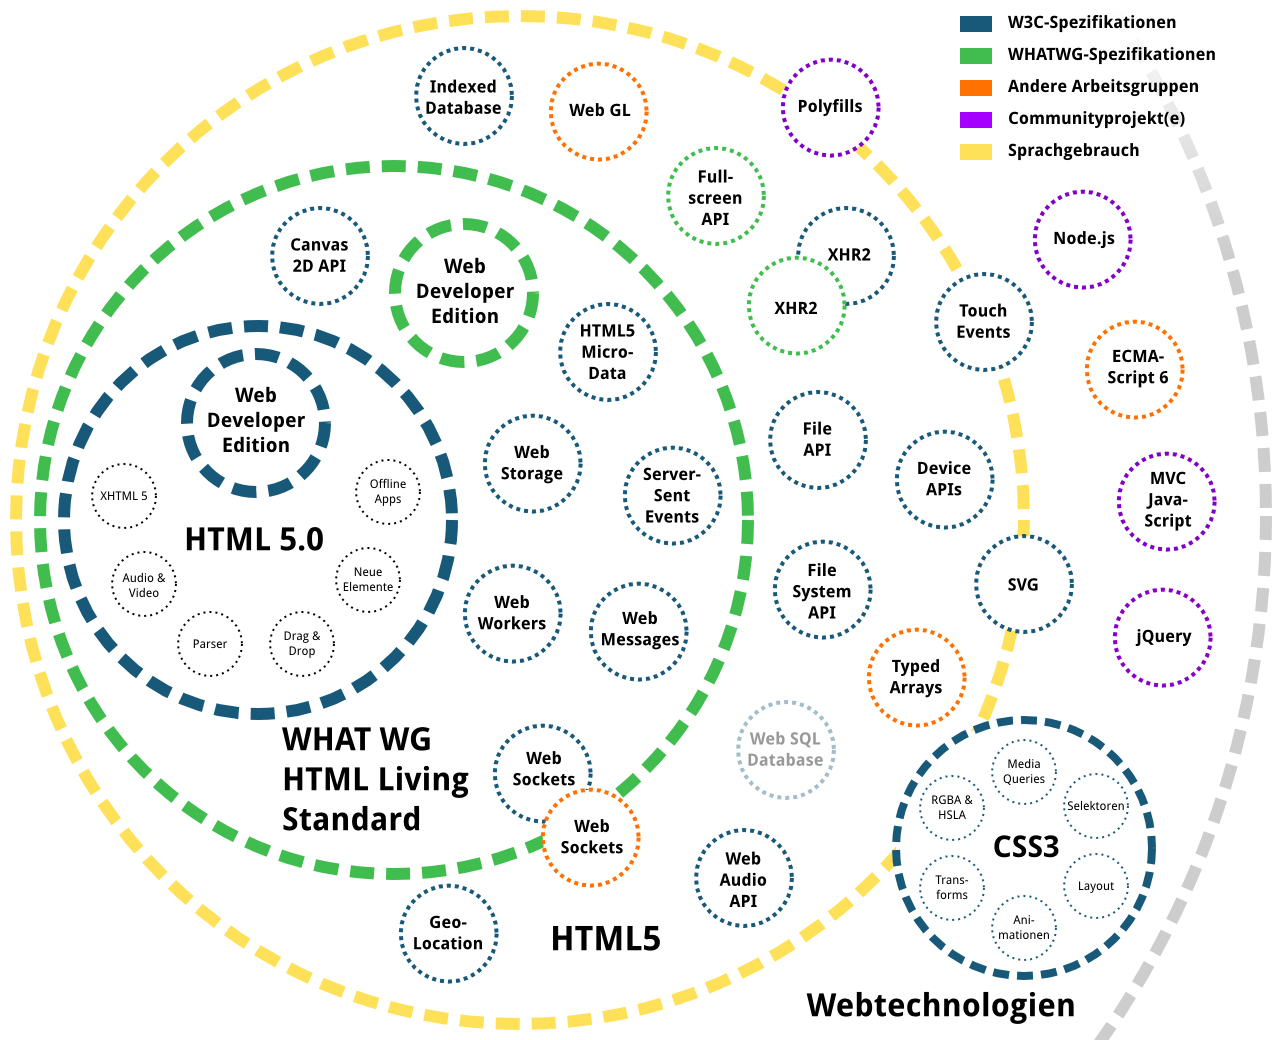
\includegraphics[width=0.75\linewidth]{abb/html5_specs}
  \caption[HTML 5 Spezifikationen Übersicht]{HTML 5 Spezifikationen Übersicht \cite{PeteKroe2014}}
  \label{fig:html5specs}
\end{figure}

\subsubsection{Ziele} HTML 5 wurde mit besonderem Augenmerk auf die Kompatibilität entwickelt. Vorhandene Spezifikationen wie HTML 4.01, XHTML 1.0 und DOM 2 sollten unter einem Dach gebündelt werden. Hierdurch wird der vorangegangenen Fragmentierung entgegen gewirkt. Schon vorhandene Inhalte müssen weitestgehend unterstützt werden auch wenn sie nicht zur HTML 5 Spezifikation gehören. Beispielsweise werden fehlerhaft verschachtelte Elemente trotzdem akzeptiert. \textit{Graceful degradation} ist als ein weiteres Ziel für HTML 5 definiert worden und bedeutet soviel wie \glqq Schrittweise Abstufung\grqq{}. Es stellt sicher, dass ein HTML Dokument auch dann verarbeitet wird sollte der verwendete Browser ein bestimmtes benutztes Element nicht unterstützen. Weiter galt für die Spezifikation, dass schon vorhandene Techniken, die weitläufig verbreitet sind, nicht neu entwickelt werden sollten. Stattdessen sollten sie übernommen werden. Dies beruht auf dem Umstand, dass die Browser Hersteller jeweils ihre eigenen Techniken bevorzugen und weiter entwickeln und dadurch auch für ihre Verbreitung sorgen. Evolution statt Revolution stand über den Zielen von HTML 5. (X)HTML wurde weiter entwickelt und nicht von Grund auf neu definiert. So ist in Tabelle \ref{tab:html5browserkomp} die zum aktuellen Zeitpunkt verfügbare Unterstützung von HTML 5 in den gängigsten Browsern abzulesen.

\vspace{1em}
\begin{center}
  \begin{tabular}{ | l | l | c | }
    \hline
    \textbf{Hersteller} & \textbf{Desktop/Mobile} & \textbf{Version} \\ \hline \hline
    Mozilla & Firefox & 4.0\\
	\hline
	& Firefox Mobile & 16\\
	\hline
	Google & Chrome & 10\\
	\hline
	& Chrome Mobile & 25\\
	\hline
	& Android & 4.0\\
	\hline
	Apple & Safari & 5.1\\
	\hline
	& Safari iOS & 5.1\\
	\hline
	Microsoft & Internet Explorer & 10\\
	\hline
	& Windows Phone & 8\\
	\hline
	Opera Software & Opera & 11.64\\
	\hline
	Blackberry & Browser & 10\\
    \hline
  \end{tabular}
\captionof{table}{HTML 5 Browserkompatibilität}
\label{tab:html5browserkomp}
\end{center}

\subsubsection{Aufbau} Ein jedes HTML Dokument beginnt mit dem sogenannten \texttt{doctype}. Dieser legt fest mit welcher Syntax das Dokument aufgebaut ist und wie das Dokument vom Browser verarbeitet werden soll. Verschiedene Varianten wie \textit{strict},\textit{transitional} und \textit{frameset} sind in HTML 5 nicht vorgesehen. In den Vorgängerversionen musste die Variante jedoch mit angegeben werden um eine eindeutige Interpretation des Dokuments zu gewährleisten. Listing \ref{lst:html401doctype} zeigt die beiden \texttt{doctype} von HTML 4.01 und XHTML 1.0. Durch die Abwärtskompatibilität von HTML 5 ist auch dieser \texttt{doctype} heute noch gültig und das Dokument wird korrekt vom Parser interpretiert werden.
    
\vspace{1em}
\begin{lstlisting}[language=HTML5, caption=(X)HTML4.01 \texttt{doctype}-Element, label=lst:html401doctype]
<!DOCTYPE HTML PUBLIC "-//W3C//DTD HTML 4.01//EN"
  "http://www.w3.org/TR/html4/strict.dtd">
<!DOCTYPE HTML PUBLIC "-//W3C//DTD HTML 4.01 Transitional//EN"
  "http://www.w3.org/TR/html4/loose.dtd">
<!DOCTYPE HTML PUBLIC "-//W3C//DTD HTML 4.01 Frameset//EN"
  "http://www.w3.org/TR/html4/frameset.dtd">        
<!DOCTYPE html PUBLIC "-//W3C//DTD XHTML 1.0 Strict//EN"
  "http://www.w3.org/TR/xhtml1/DTD/xhtml1-strict.dtd">    
\end{lstlisting}
	
Listing \ref{lst:html5doctype}	hingegen zeigt das \texttt{doctype} von HTML 5. Es wurde enorm gekürzt im Vergleich zu dem \texttt{doctype} von HTML 4.01 und XHTML 1.0. Groß- und Kleinschreibung ist nicht von Bedeutung innerhalb des \texttt{doctype}. 

\vspace{1em}
\begin{lstlisting}[language=HTML5, caption=HTML 5 \texttt{doctype}-Element, label=lst:html5doctype]
<!DOCTYPE html>
\end{lstlisting}		
	
Nach dem \texttt{doctype} folgt der restliche Dokument Aufbau in HTML Syntax. Diese teilt sich auf in Elemente und Attribute, die diesen Elementen zugeordnet und mit Werten versehen werden können. Es existieren für die meisten Elemente Start- und Endmarkierungen. Für einige Elemente sind die Start- bzw. Endmarkierungen optional und für einige wiederum verpflichtend in der Dokumentstruktur zu setzen. In Listing \ref{lst:html5basicdoc} sieht man ein valides HTML 5 Dokument mit den Grund Elementen für eine komplett leere Seite.(vgl. \cite[S.58]{KronHTML2011})

\vspace{1em}
\begin{lstlisting}[language=HTML5, caption=HTML 5 Basis Dokument, label=lst:html5basicdoc]
<!DOCTYPE html>
<html>
 <head>
   <title>Beispieltitel</title>
 </head>
 <body>
   <h1>Ueberschrift 1</h1>
 </body>
</html>
\end{lstlisting}
	
\subsubsection{Wichtige neue Sprachelemente} In HTML 5 wurden die Mikrodaten mit aufgenommen. Mit Mikrodaten bietet sich eine weitere Möglichkeit ein HTML Dokument semantisch zu spezifizieren. Metadaten wie z.B. der verwendete Zeichensatz lassen sich so festlegen. Browser und Webseiten können über die Mikrodaten-API die gesetzten Werte auslesen und weiter verarbeiten. Auch Suchmaschinen können auf die Metadaten zugreifen, verwenden sie jedoch heutzutage weitestgehend nicht mehr. Aus diesem Grund tragen die Metadaten zwar zur semantischen Struktur des HTML bei, können aber aus Sicht der Suchmaschinenoptimierung getrost vernachlässigt werden.(vgl. \cite{SelfHtml20142}) Weiter kann man bei Mikrodaten davon sprechen, \glqq [...] dass sie auf Name/Werte-Paaren basieren. Jedes Mikrodatenvokabular definiert eine Menge benannter Eigenschaften.\grqq{}(vgl. \cite[S.174]{PilgDurc2011}) Listing \ref{lst:html5meta} zeigt Beispielhaft das \texttt{head}-Element eines HTML Dokuments mit vier, darin eingeschlossenen, \texttt{meta}-Elementen. Unter anderem wird mit dem ersten \texttt{meta}-Element der Zeichensatz näher definiert. Das \texttt{meta}-Element mit Namen \texttt{viewport}, dient dazu die Skalierung auf Mobilgeräten zu unterdrücken, damit die Seite sich an den \texttt{viewport} anpasst.

\vspace{1em}
\begin{lstlisting}[language=HTML5, caption=HTML 5 \texttt{meta}-Element, label=lst:html5meta]
<head>
  <meta charset="utf-8">
  <meta name="viewport" content="width=device-width;" />
  <meta name="keywords" content="Lorem ipsum">
  <meta name="author"   content="dolor sem it">
</head>
\end{lstlisting}
		
Zwei weitere neue Elemente in HTML 5 sind das \texttt{header}- und \texttt{footer}-Element. Üblich ist es im \texttt{header}-Element einer Website Komponenten wie das Logo, das Menü und den Titel unterzubringen. Im \texttt{footer}-Element dagegen werden Kontakt, Impressum und das Copyright aufgeführt. In Listing \ref{lst:html5header} ist die Platzierung des \texttt{header}- und \texttt{footer}-Elements innerhalb eines \texttt{body}-Elements einer Webseite zu sehen.

\vspace{1em}
\begin{lstlisting}[language=HTML5, caption=HTML 5 \texttt{header}- und \texttt{footer}-Element, label=lst:html5header]
<body>
  <header>
    <img src="logo.gif" alt="logo">
    <h1>Ueberschrift</h1>
  </header>
  <footer>
     <a href="kontakt.html">Kontakt</a>
  </footer>
</body>
\end{lstlisting}
	
Um ein HTML Dokument nach heutigen Maßstäben korrekt zu strukturieren wurden einige Elemente der Spezifikation hinzugefügt. So lässt sich die Navigation nun mit dem \texttt{nav}-Element umschließen wie in Listing \ref{lst:html5struct} ab Zeile 3 zu sehen. \glqq Das \texttt{section}-Element repräsentiert einen allgemeinen Abschnitt in einem Dokument oder einer Anwendung. Ein Abschnitt ist in diesem Kontext eine thematische Gruppierung von Inhalten, die üblicherweise unter einer Überschrift stehen. Beispiele für Abschnitte wären Kapitel, die verschiedene Tabs in einem Dialog mit Tabs oder die nummerierten Abschnitte einer wissenschaftlichen Arbeit.[...] Das \texttt{article}-Element repräsentiert eine abgeschlossene Einheit in einem Dokument, einer Anwendung oder einer Site, die unabhängig verbreitet oder wiederverwendet werden kann, z.B. in RSS-Feeds. Es könnte beispielsweise ein Forenbeitrag, ein Zeitschriften- oder Zeitungsartikel, ein Blog-Eintrag, ein Benutzerkommentar, ein interaktives Widget oder Gadget oder ein Element mit unabhängigem Inhalt enthalten.

\vspace{1em}
\begin{lstlisting}[language=HTML5, caption=HTML 5 Struktur Elemente, label=lst:html5struct]
<body>
  <header>
    <nav>
      <ul>
        <li><a href="#link_1.html">Wiki</a></li>
        ...
      </ul>
    </nav>
  </header>
  <main>
  <article>
    <h1>Ueberschrift</h1>
    <p>Dies ist eine Beispiel HTML 5-Seite</p>
  </article>
  <aside>
    <section>
      <h2>Kontakt</h2>
      <ul>
        <li><a href="link_1.html">Wiki</a></li>
        ...
      </ul>
    </section>
  </aside>
  </main>
  <footer>
  </footer>
</body>
\end{lstlisting}
	
Das \texttt{aside}-Element repräsentiert einen Abschnitt einer Seite, der Inhalte enthält, die sich zwar auf den das \texttt{aside}-Element umgebenden eigentlichen Inhalt der Seite beziehen, aber als von ihm unabhängig betrachtet werden können. In Druckwerken werden derartige Abschnitte häufig als Seitenleisten dargestellt. Das Element kann für typografische Effekte wie herausgehobene Zitate oder Seitenleisten, für Werbung, für Gruppen von \texttt{nav}-Elementen und andere Inhalte verwendet werden, die als vom eigentlichen Inhalt der Seite getrennt betrachtet werden können.\grqq{}\cite[S.43]{PilgDurc2011} Das neue \texttt{main}-Element ist zur Auszeichnung des Seitenhauptinhalts vorgesehen. Mit dieser Auszeichnung lässt sich z.B. mit Screenreadern direkt zum Hauptinhalt springen.  Alle genannten Elemente sind in Listing \ref{lst:html5struct} in ihrer vorgesehenen Reihenfolge abgebildet. \glqq Damit auch ältere Internet Explorer der Versionen 6-8 die neuen HTML 5-Elemente darstellen können, kann ein kurzes JavaScript eingebunden werden. Am einfachsten ist es, dieses nicht auf dem eigenen Server vor zuhalten, sondern direkt von Google abzurufen. Dies hat überdies den Vorteil, dass es oft schon im Browser-Cache der Nutzer vorhanden ist. Der Aufruf erfolgt in einem \textit{Conditional Comment}, der nur vom Internet Explorer kleiner als Version 9 (lt IE 9) verstanden wird. Alle andere Browser ignorieren dies als reinen Kommentar.\grqq{}\cite{SelfHtml20143} In Listing \ref{lst:html5fallback}	 ist der beschriebene Rückfallmechanismus verdeutlicht.

\vspace{1em}
\begin{lstlisting}[language=HTML5, caption=HTML 5 Internet Explorer Fallback, label=lst:html5fallback]
<head>
  <meta charset="utf-8">
  <!--[if lt IE 9]>
  <script src="http://goo.gl/RfQF7"></script>
  <![endif]-->
  <title>HTML 5-Seite mit Grundstruktur</title>
</head>
\end{lstlisting}
	
Eingabefelder sind in den meisten Applikationen unabdingbar. Aus diesem Grund wurden in HTML 5 eine viel zahl an \texttt{input}-Elementen hinzugefügt. So müssen keine komplizierten Workarounds mit JavaScript oder anderen Skriptsprachen mehr verwendet werden. \glqq Das typische HTML 5-Formular unterscheidet sich nicht fundamental von seinen in HTML 4.01 oder XHTML 1 geschriebenen Gegenstücken. Alle alten Formularelemente sind noch da und verhalten sich weitgehend wie bisher. Die Neuerungen bestehen aus einigen neuen Funktionen, Attributen und APIs und aus einer ganzen Reihe neuer möglicher Werte für das \texttt{type}-Attribut des \texttt{input}-Elements.\grqq{}\cite[S.176]{KronHTML2011} In Listing \ref{lst:html5input} sind beispielhaft einige neue Werte des \texttt{type}-Attributs ausgeführt. Eingabefelder des Typs \texttt{tel, email} oder \texttt{url} sind vom Verständnis her simple Texteingabefelder. Als wichtige Besonderheit lässt sich bei \texttt{email}- und \texttt{url}-Feldern aber ihre eingebaute Validation nennen. Verwendet man die Validierungs-API werden nur korrekte URLs bzw. E-Mails zugelassen. Für ein \texttt{tel}-Feld gilt dies nicht. Außerdem wird auf Smartphones und Tablet-Geräten die angezeigte Bildschirmtastatur entsprechend des erwarteten Eingabetyps für eine optimale Eingabe angepasst dargestellt.(vgl. \cite[S.178]{KronHTML2011}) So wird bei einer erwarteten E-Mail Adresse das @-Symbol direkt auf der Bildschirmtastatur als eigene Taste mit angezeigt, was normalerweise nicht der Fall ist. Einige der neuen Elementausprägungen besitzen noch zusätzliche Attribute die die Eingabemöglichkeit weiter einschränken und präzisieren können. Zu sehen in Zeile 5 von Listing \ref{lst:html5input} im \texttt{time}-Feld, bei dem die erwartete Zeit von 9:00 Uhr bis 17:00 Uhr nur einstellbar ist. \texttt{input}-Elemente können über das \texttt{required}-Attribut außerdem als Pflichtfeld markiert werden.

\vspace{1em}
\begin{lstlisting}[language=HTML5, caption=HTML 5 \texttt{input}-Element, label=lst:html5input]
<body>
  <input type="tel">
  <input type="email">
  <input type="url">  
  <input type="time"  min="09:00" max="17:00">
  <input type="date"  required="required">
</body>
\end{lstlisting}
	
Für multimediale Inhalte auf Webseiten wurden der Spezifikation passende Elemente hinzugefügt. Das \texttt{canvas}-Element \glqq [...] stellt eine Fläche zur Verfügung, auf die mittels JavaScript dynamische Bitmap-Grafiken gezeichnet werden können. So lassen sich Animationen erstellen, Diagramme zeichnen, eigene Interface-Elemente kreieren und Videos manipulieren\grqq{}\cite[S.353]{KronHTML2011} Für Audio und Video Inhalte wurden die gleichnamigen Elemente geschaffen. 
	
\subsection{CSS 3}
Das Kapitel CSS 3 erläutert kurz die Notwendigkeit von CSS und geht dann weiter auf die Einbindung in einem HTML Dokument ein. Anschließend wird die Syntax der Gestaltungssprache beschrieben. Einige Eigenheiten wie Selektoren und Pseudoklassen werden erklärt um dann zum Box-Modell zu kommen. Abgerundet wird das Kapitel mit der Definition der spezifischen Stylesheets, die gerade in der Web Entwicklung ihre Stärken zeigen.

\subsubsection{Einleitung}
\glqq Cascading Style Sheets (CSS) bieten mächtige Möglichkeiten, die Präsentation eines Dokuments oder einer Sammlung von Dokumenten zu beeinflussen. Offensichtlich ist CSS ohne irgendein Dokument ziemlich nutzlos, da es keine Inhalte zu präsentieren gäbe.\grqq{}\cite[S.1]{MeyeCasc2005} CSS gehört mit zu den Kernsprachen des WWW. \glqq Zuallererst ermöglicht CSS eine wesentlich umfangreichere Gestaltung des Aussehens eines Dokuments, als HTML das jemals konnte, nicht einmal als die Präsentationselemente einen Großteil der Sprache ausmachten. Mit CSS kann für jedes Element eine eigene Text- und Hintergrundfarbe festgelegt werden. Jedes Element lässt sich zudem mit einem Rahmen versehen; der Platz um ein Element herum kann in der Größe verändert werden und es kann Einfluss auf die Groß- und Kleinschreibung genommen werden. Mit CSS können Sie außerdem  bestimmen, wie fett bestimmte Textteile dargestellt werden sollen, welche Dekoration (z.B. Unterstreichungen) verwendet werden soll, wie groß die Abstände zwischen einzelnen Buchstaben und Wörtern sein sollen und ob der Text überhaupt angezeigt wird.\grqq{}\cite[S.4]{MeyeCasc2005}

\subsubsection{Einbindung} Um eine Webseite überhaupt mit CSS zu gestalten muss es innerhalb eines HTML Dokuments eingebunden sein. Dies ist auf drei verschiedene Arten möglich. Als Erstes mal das \texttt{link}-Element. \glqq CSS benutzt dieses Tag, um Stylesheets mit dem Dokument zu verbinden.[...] Stylesheets, die nicht im HTML-Dokument selbst enthalten sind, sondern von außen eingebunden werden, bezeichnet man als externe Stylesheets[...].Um ein Stylesheet erfolgreich zu laden, muss sich ein \texttt{link} innerhalb des \texttt{head}-Elements befinden, darf aber nicht innerhalb eines anderen Elements wie etwa \texttt{title} stehen.\grqq{}\cite[S.14]{MeyeCasc2005} In Listing \ref{lst:css3einbindunglink} ist die Einbindung eines externen Stylesheets über das \texttt{link}-Element zu sehen.
	
\vspace{1em}
\begin{lstlisting}[language=HTML5, caption=Stylesheet Einbindung über \texttt{link}-Element, label=lst:css3einbindunglink]
<head>
  <link rel="stylesheet" type="text/css" href="beispiel.css" />
</head>
\end{lstlisting}

Eine andere Möglichkeit ist es das CSS direkt innerhalb eines \texttt{style}-Elements zu positionieren. Ein Element vom Typ \glqq \texttt{style} sollte immer zusammen mit dem Attribut \texttt{type} verwendet werden. Im Fall eines eingebetteten CSS-Dokuments ist der korrekte Wert \glqq \texttt{text/css}\grqq, genau wie bei dem Element \texttt{link}.[...] Die Stildefinition zwischen den öffnenden und schließenden \texttt{style}-Tags bezeichnet man als Dokumenten-Stylesheet oder auch als eingebettetes Stylesheet[...].\grqq{}\cite[S.19]{MeyeCasc2005} Listing \ref{lst:css3einbindungstyle} zeigt ein solches eingebettetes Stylesheet.

\vspace{1em}
\begin{lstlisting}[language=HTML5, caption=Stylesheet Einbindung über \texttt{style}-Element, label=lst:css3einbindungstyle]
<head>
	<title>Dokument mit Formatierungen</title>
	<style type="text/css">
		body { color: purple; background-color: #d8da3d; }
	</style>
</head>
\end{lstlisting}
	
Als letzte Möglichkeit kann man ein Stylesheet bzw. Style-Informationen direkt einem HTML Element anhängen. \glqq Durch das direkte Festlegen von Formaten, umgangsprachlich auch \glqq Inline-Style\grqq{} genannt, gehen viele Vorteile verloren. Der Wartungsaufwand steigt während die Flexibilität sich verringert. Inline-Styles sind an ein Dokument gebunden und können nicht an zentraler Stelle bearbeitet werden.\grqq{}\cite{SelfHtml20144} In Listing \ref{lst:css3einbindunghtml} wird dem \texttt{span}-Element ein \glqq Inline-Style\grqq gegeben.

\vspace{1em}
\begin{lstlisting}[language=HTML5, caption=Stylesheet Einbindung in \texttt{html}-Element, label=lst:css3einbindunghtml]
<span style="font-size: small;">Text</span>
\end{lstlisting}
	
Innerhalb von CSS-Dateien kann man wiederum mit der Direktive \texttt{@import} den Browser dazu zu bringen weitere Stylesheets nachzuladen und zu verwenden. Zu beachten ist, dass die \texttt{@import} Direktive vor allen anderen CSS Befehlen steht, bei den eingebetteten wie auch den externen Stylesheets.(vgl. \cite[S.20]{MeyeCasc2005})

\subsubsection{Syntax} Die Syntax von CSS ist denkbar einfach. Sie besteht im wesentlichen aus dem Selektor und dem Deklarationsblock. Ein Selektor entspricht in den häufigsten Fällen dem gleichnamigen HTML Element. Der Deklarationsblock wiederum besteht aus mindestens einer Deklaration.(vgl. \cite[S.26]{MeyeCasc2005}) \glqq Eine Deklaration besteht dabei immer aus einer Eigenschaft, die mit einem Wert durch einen Doppelpunkt verbunden ist. Abgeschlossen wird die Deklaration durch ein nachgestelltes Semikolon. Auf den Doppelpunkt und das Semikolon kann eine beliebige Anzahl von Leerzeichen (also auch keines) folgen. Fast immer besteht der Wert aus einem einzelnen Schlüsselwort oder einer durch Leerzeichen getrennten Liste aus mehreren Schlüsselwörtern, die für die genannte Eigenschaft zulässig sind.\grqq{}\cite[S.28]{MeyeCasc2005} Verwendet man in der Deklaration ungültige Eigenschaften oder Werte werden diese einfach ignoriert. Listing \ref{lst:css3syntax} zeigt die Syntax beispielhaft.

\vspace{1em}
\begin{lstlisting}[language=CSS, caption=CSS3 Syntax Beispiel, label=lst:css3syntax]
Selektor [, Selektor2, ...] {
  Eigenschaft1: Wert1;
  ...
  EigenschaftN: WertN[;]
}
\end{lstlisting}

Um sich wiederholende Design Regeln zusammenfassen zu können lassen sich Selektoren in CSS gruppieren. Dabei werden die zu gruppierenden Selektoren durch ein Komma von einander getrennt und dann die zu gestaltenden Eigenschaften mit den entsprechenden Werten genannt wie in Listing \ref{lst:css3group} zu sehen.

\vspace{1em}
\begin{lstlisting}[language=CSS, caption=CSS3 Gruppierung, label=lst:css3group]
h1, h2, p {
  color: black;
}
\end{lstlisting}

\subsubsection{Selektoren} CSS arbeitet wie HTML auch mit dem DOM. \glqq Der erste Vorteil, der sich aus dem Verständnis dieses Modells ergibt, ist die Möglichkeit, Selektoren für Nachfahren (auch als Kontext-Selektoren bezeichnet) zu definieren. Die Definition von Selektoren für Nachfahren besteht aus dem Festlegen von Regeln, die nur für bestimmte hierarchische Strukturen gelten.\grqq{}\cite[S.48]{MeyeCasc2005} Der erst genannte Selektor ist das Elternelement. Mittels eines Leerzeichens wird das Nachfahren Element vom Elternelement getrennt. In Listing \ref{lst:css3kids} wird angegeben, dass jedes \texttt{strong}-Element innerhalb eines \texttt{h1}-Elements eine besondere Formatierung erhält. Konkret bedeutet das in diesem Fall, dass die Schriftgröße 14pt und die Schriftgewichtung, welche die Dicke und Stärke festlegt, \texttt{bold} sein soll. Zu beachten ist, dass so sämtliche Nachfahren des \texttt{h1}-Elements entsprechend formatiert werden. Es gibt auch die Möglichkeit die Formatierung nur auf einen direkt Nachfahren, ein sogenanntes Kindelement, zu beschränken. Um dies zu erreichen werden Eltern- und Kindelement nicht durch ein Leerzeichen von einander getrennt, sondern durch das Größer-als-Zeichen (\textgreater).

\vspace{1em}
\begin{lstlisting}[language=CSS, caption=CSS3 Selektoren für Nachfahren, label=lst:css3kids]
h1 strong {
  font-size:  14pt;
  font-weight: bold;  
}
\end{lstlisting}

Das gleiche Verfahren kann auch auf Nachbarelemente angewandt werden. Nur wird hierbei ein anderes Kombinatorenzeichen benötigt, nämlich das Plus (+).\\
\glqq Zusätzlich zu den rohen Dokument-Elementen gibt es noch zwei weitere Arten von Selektoren: Klassenselektoren und ID-Selektoren, mit denen sich Stildefinitionen unabhhängig von den Elementen eines Dokuments zuweisen lassen. Diese Selektoren können eigenständig oder zusammen mit Elementselektoren verwendet werden. Allerdings ist es hierfür notwendig, die Dokumentteile entsprechend zu markieren. Die Benutzung dieser neuen Selektoren erfordert daher [...] Voraussicht und Planung.\grqq{}\cite[S.34ff]{MeyeCasc2005} Des weiteren muss die HTML Auszeichnung angepasst werden sollten Klassen- und/oder ID-Selektoren verwendet werden. Konkret bedeutet dies, dass jedem HTML Element ein \texttt{class}- und/oder \texttt{id}-Attribut hinzugefügt werden muss sofern es von den CSS Regeln beachtet werden soll. Zu beachten ist, dass eine vergebene ID im gesamten HTML Dokument einzigartig sein muss, wohingegen eine vergebene Klasse auf mehrere HTML Elemente und auf ein HTML Element auch mehrere Klassen angewandt werden können. (vgl. \cite{W3ScCss2014}) Listing \ref{lst:css3idclass} zeigt einen solchen ID-Selektor, einen Klassenselektor und einen Klassenselektor der nur auf \texttt{p}-Elementen gilt die das \texttt{class}-Attribut besitzen.

\vspace{1em}
\begin{lstlisting}[language=CSS, caption=CSS3 Klassen- und ID-Selektoren, label=lst:css3idclass]
<div id="ID">
  <p class="Klasse"></p>
</div>

div#ID {
  text-align: center;
  color:      red;
}
.Klasse {
  text-align: center;
  color:      red;
}
p.Klasse {
  text-align: center;
  color:      red;
}
\end{lstlisting}
	
\subsubsection{Pseudoklassen} Neben den genannten gibt es noch einen weiteren Typ von Selektoren. Die sogenannten Pseudoselektoren für die Pseudoklassen. \glqq Mit diesen Selektoren [... kann man] Stildefinitionen auf Strukturen zuweisen, die nicht unbedingt im Dokument vorkommen müssen, oder auch [... Pseudo]klassen, die vom Zustand bestimmter Elemente oder sogar vom Zustand des Dokuments selbst abhängen. Anders gesagt, werden die Stile, basierend auf etwas anderem als der Struktur des Dokuments, auf Teile des Dokuments angewendet.\grqq{}\cite[S.53ff]{MeyeCasc2005} Um beispielsweise einen Link in einem Dokument farblich zu markieren sobald er besucht wurde wäre eigentlich für jeden Zustand des Links eine eigene Klasse nötig. Diese Klasse müsste sich ständig ändern je nach dem ob der Nutzer den Link schon besucht hat oder nicht. Um diesen Umstand zu verhindern existieren die Pseudoselektoren und Pseudoklassen. Im Fall eines \texttt{a}-Elements werden die Pseudoklassen \texttt{link} und \texttt{visited} bereitgestellt um den Effekt zu erzeugen. Diese Klassen werden dem \texttt{a}-Element durch CSS selber hinzugefügt bzw. wird ein \texttt{a}-Element, das ein \texttt{href}-Attribut besitzt und noch nicht besucht wurde mit der Pseudoklasse \texttt{link} versehen. Die Pseudoklasse \texttt{visited} bezieht sich auf \texttt{a}-Elemente mit \texttt{href}-Attribut die schon besucht wurden. Listing \ref{lst:css3pseudo} zeigt ein solches \texttt{a}-Element und die beiden Pseudoselektoren.

\vspace{1em}
\begin{lstlisting}[language=CSS, caption=CSS3 Pseudoklassen und -selektoren, label=lst:css3pseudo]
<a href="http://www.example.com">Example.com</a>

/* unvisited link */
a:link {
  color: #FF0000;
}

/* visited link */
a:visited {
  color: #00FF00;
}
\end{lstlisting}

\subsubsection{Box-Modell} \glqq CSS geht davon aus, dass jedes Element eine oder mehrere rechteckige Boxen erzeugt, die Element-Boxen genannt werden.[...] Im Kern besitzt jede Box einen Inhaltsbereich (content area). Dieser wird umgeben von optionalen Innenabständen (padding), Rahmen (borders) und Außenabständen (margins). Diese Teile werde als optional angesehen, weil sie alle eine Breite von null Einheiten haben können, also sozusagen nicht vorhanden sind.\grqq{}\cite[S.167]{MeyeCasc2005} \glqq Da eine Box aus mehreren Komponenten bestehen kann, werden für die einzelnen Bereiche verschiedene Kantenbezeichnungen definiert. Als Innen- oder Inhaltskante wird die Strecke bezeichnet, die den Inhaltsbereich einer Box umfasst. Das ist der Bereich, der durch den Inhalt oder die Eigenschaften \texttt{width} und \texttt{height} festgelegt wurde. Der Bereich einer Box, der von den Innenkanten umgeben ist, wird auch \textit{content box} (Inhaltsbox) genannt. Die Kanten, die eine Box mitsamt Innenabstand umfassen, werden Polsterungskanten genannt. Der von diesen Kanten umfasste Bereich wird \textit{padding box} (Polsterungsbox) genannt. Besitzt eine Seite keinen Innenabstand, so ist die Polsterungskante mit der Innenkante identisch. Die Rahmenkanten umgeben eine Box mit deren Rahmen. Der durch diese Kanten abgesteckte Bereich wird \textit{border box} (Rahmenbox) genannt. Besitzt eine Box keinen Rahmen, so ist die Rahmenkante mit der Polsterungskante identisch. Eine vollständige Box wird durch die Außenkanten definiert. Die Außenkante umfasst eine Box mitsamt Außenabständen, also die \texttt{margin box}. Sind für eine Box keine Außenabstände definiert, so ist die Außenkante mit der Rahmenkante identisch.\grqq{}\cite{SelfHtml20145}\\Die Gesamtbreite eines Elements definiert sich dadurch als Summe aus Breite, linkem und rechtem Innenabstand, linkem und rechtem Rahmen und dem linkem und rechtem Außenabstand. Für die Gesamthöhe verhält sich die Berechnung analog. Abbildung \ref{fig:cssboxmodell} zeigt das beschriebene CSS-Box-Modell.

\vspace{1em}
\begin{figure}[htb]
  \centering
  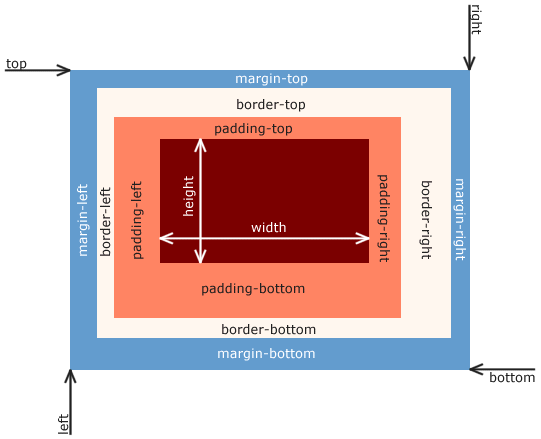
\includegraphics[width=0.8\linewidth]{abb/css_boxmodell}
  \caption[CSS-Boxmodell]{CSS-Boxmodell\cite{WikiCSS2014}}
  \label{fig:cssboxmodell}
\end{figure}	
	
\subsubsection{Spezifische Stylesheets} \glqq Dank der Mechanismen in CSS und HTML [... lassen sich] beliebige Stylesheets auf bestimmte Medien beschränken. In HTML-basierten Stylesheets geschieht dies mit Hilfe des Attributs \texttt{media} und gilt sowohl für \texttt{link}- wie auch \texttt{style}-Elemente. Das Attribut \texttt{media} akzeptiert entweder die Angabe eines einzelnen Mediums oder eine durch Komma getrennte Liste von Werten.\grqq{}\cite[S.434ff]{MeyeCasc2005} Die Angaben in Listing \ref{lst:css3media} bewirken eine gesonderte Formatierung für ein \texttt{print} Medium.

\vspace{1em}
\begin{lstlisting}[language=HTML5, caption=CSS3 medienspezifisches Stylesheet, label=lst:css3media]
<link rel="stylesheet" type="text/css" media="print" href="print.css">
\end{lstlisting}
	
Ein vorhandenes Stylesheet ohne Medieninformationen gilt für alle Medien. Fernen lassen sich die Medien auch innerhalb des Stylesheets näher beschreiben durch den \texttt{@media}-Block. Diesen \texttt{@media}-Blöcken können neben den Medientypen auch noch weitere Bedingungen hinzugefügt werden. In Listing \ref{lst:css3mediaquery} wird das Element mit der ID \texttt{inhalt} auf eine Breite von \texttt{800px} festgelegt. Ist das verwendete Ausgabemedium jedoch ein Bildschirm und hat nur eine Gesamtbreite von \texttt{1024px} wird das Element mit der ID \texttt{inhalt} auf eine Breite von nur noch \texttt{600px} und das \texttt{aside}-Element gar nicht mehr angezeigt.

\vspace{1em}
\begin{lstlisting}[language=CSS, caption=CSS3 eigenschaftsspezifisches Stylesheet, label=lst:css3mediaquery]
#inhalt {
	width: 800px;
}
 
@media screen and (max-width: 1024px) {
	#inhalt {
		width: 600px;
	}
	aside {
		display: none;
	}
}
\end{lstlisting}

\subsection{JavaScript}
Dieses Kapitel soll ein grundlegendes Verständnis für die Skriptsprache JavaScript aufbauen. Beginnend mit der Historie und dem Sandbox-Prinzip hin zur Objektorientierung und den Sprachelementen werden außerdem die einzelnen Datentypen, Werte und Variablen beschrieben. Im Detail werden dann die Operatoren, Schleifen und Kontrollstrukturen erörtert und durch Listings verdeutlicht. Des Weiteren ist das Document-Object-Modell, die Ereignisverarbeitung und AJAX wichtig zum Verständnis des Frameworks jQuery, auf welchem letztendlich auch das SAP UI 5 Framework basiert.

\subsubsection{Historie} JavaScript wurde 1995 von Netscape entwickelt, lizenziert und eingeführt. Um der Sprache von Anfang an einen Standardcharakter zu geben wurde die Organisation ECMA hinzugezogen. Die ECMA veröffentlichte unter dem Namen ECMAScript einen, auf Netscapes JavaScript Spezifikation basierenden, Industriestandard der Sprache. Da JavaScript somit eine proprietäre Sprache von Netscape ist, hat Microsoft seine eigene Variante, mit Namen JScript, veröffentlicht. JScript implementiert JavaScript vollständig, besitzt allerdings auch noch Zusatzfunktionen wie z.B. Zugriff auf das Dateisystem und das Betriebssystem Windwos. Mit Version 1.5 von JavaScript erhielt das DOM Einzug in die Implementierung. Da jeder Browser seinen eigenen JavaScript Interpreter besaß, war es kaum Möglich einheitlichen Code für alle Browser zu entwickeln. Es musste auf alle Eventualitäten geachtet werden. Um diesem Missstand entgegen zu wirken wurde das W3C hinzugezogen um einen einheitlichen Sprachstandard zu etablieren. Jedoch entwickelte das W3C keinen konkreten JavaScript-Standard, sondern eine Schnittstelle - das erwähnte DOM. Die aktuelle JavaScript Version von 2010 ist 1.8.5 und ECMAScript liegt in Version 5.1 seit Juni 2011 vor. (vgl. \cite{SelfHtml20146})

\subsubsection{Sandbox-Prinzip} JavaScript wird innerhalb eines Browser in einer sogenannten Sandbox ausgeführt. Das bedeutet es liegt in einem abgesichertem Speicherbereich, aus welchem es keinen Zugriff auf Objekte außerhalb des Browsern hat. Eine Ausnahme ist der Lesezugriff auf Dateien die mittels des \texttt{input}-Elements von einem Nutzer selbst hoch geladen werden. Des weiteren kann mit JavaScript auch nicht ohne weiteres auf bestimmte sicherheitskritische Funktionen des ausführenden Browser zugegriffen werden. Um beispielsweise das Browserfenster zu schließen, Symbolleisten ein- und auszublenden oder zugriff auf die Seitenhistorie zu erlangen sind Nutzereingaben nötig. (vgl. \cite{WikiJS2014})

\subsubsection{Paradigma} \glqq JavaScript gehört zu den sogenannten objektorientierten Programmiersprachen (oder, um genauer zu sein, zu den objektbasierten Sprachen). Das Konzept der objektorientierten Programmierung (OOP) wird im Folgenden sehr stark vereinfacht erklärt.[...] In JavaScript ist (mit Ausnahme der Variablen) alles, worauf man zugreift, ein Objekt. Ein Objekt ist der Versuch, die reale Welt in eine Programmiersprachenumgebung abzubilden. Ein Standardbeispiel für Objekte ist etwa ein Auto. Das Auto an sich (als abstrakter Begriff) kann als Objekt angesehen werden, ein einzelnes Auto wird als Instanz des Objekts Auto bezeichnet.\grqq{}\cite[S.93]{WenzJava2008} Ein Auto bzw. ein Objekt generell lässt sich durch Parameter näher beschreiben. Diese Parameter gibt es in zwei Ausführungen. Die Eigenschaften und die Methoden. Bei einer Eigenschaft handelt es sich im Grunde um eine Variable die einen festen Bezug zum Objekt besitzt. Eigenschaften können gelesen und gesetzt werden. Ein Auto hat beispielsweise als Eigenschaft die Anzahl der Türen oder die Motorleistung. Methoden auf der anderen Seite müssen nicht immer einen Informationswert zurückgeben. Bei dem Objekt Auto könnte es eine Methode \texttt{tunen()} geben die dann Einfluss auf die Eigenschaft Motorleistung nimmt.\\Im Kontext der Webentwicklung mit JavaScript existieren einige feste Objekte die zu jederzeit zur Verfügung stehen. Da wäre zum einen das \texttt{window}-Objekt, dass, wie der Name schon erahnen lässt, das aktuelle Browserfenster repräsentiert. Über die Eigenschaften und Methoden lassen sich Informationen zum Browserfenster erhalten und beispielsweise neue Fenster öffnen. Das \texttt{document}-Objekt bildet den Inhalt eines Browserfensters ab. Es stellt das Ausgangsobjekt für das DOM dar. Es steht in der Hierarchie direkt unter dem \texttt{window}-Objekt. Neben diesen Objekten existieren noch weitere um den Browserkontext möglichst genau innerhalb einer JavaScript Anwendung verfügbar zu machen.(vgl. \cite{SelfHtml20147})

\subsubsection{Sprachelemente} JavaScript wird mit dem Unicode Zeichensatz geschrieben. Die 16-Bit-Codierung bei Unicode enthält fast sämtliche Zeichen der Schriftsprachen der Welt. Die Nutzung von Unicode trägt wesentlich zu der Internationalisierung bei. Bei der Groß- und Kleinschreibung unterscheidet JavaScript eindeutig. So müssen alle Schlüsselwörter und Bezeichner immer in der selben vorgegebenen Schreibweise geschrieben werden, damit sie vom JavaScript Interpreter korrekt behandelt werden. Whitespace, Tabulatoren und Zeilentrenner werden vom Interpreter komplett ignoriert und können deshalb zur visuellen Strukturierung des Programmcodes genutzt werden. Dadurch kann der Programmcode leicht leserlich und verständlich formatiert werden ohne das dadurch die Logik verletzt wird. Das, aus anderen Programmiersprachen bekannte, Semikolon am Ende einer Anweisung ist in JavaScript nicht zwingend erforderlich. Eine Anweisung ist im Normalfall mit dem Ende der Zeile abgeschlossen. So muss ein Semikolon lediglich gesetzt werden, wenn sich mehr als eine Anweisung in der Zeile befinden oder eine Anweisung über mehrere Zeilen hinweg formuliert wurde. Fehlende Semikola werden vom Interpreter selbst gesetzt, was in bestimmten Fällen aber zum Bruch der Logik führen kann wie in Listing \ref{lst:jssemikolon} zu sehen.(vgl. \cite[S.15ff]{FlanJava2007})

\vspace{1em}
\begin{lstlisting}[language=JavaScript, caption=JavaScript Logikbruch Semikolon, label=lst:jssemikolon]
// kein Interpretierungsfehler
a = 3
b = 4;

// korrekte Schreibweise in einer Zeile
a = 3; b = 4;

// Interpreter setzt Semikolon automatisch
return
true;
// falsche Interpretation anschliessend
return;
true;
\end{lstlisting}

Des weiteren gibt es einige Literale in JavaScript. \glqq Ein Literal ist ein Datenwert, der direkt in einem Programm vorkommt. Literale können zum Beispiel folgendermaßen aussehen:\grqq{}\cite[S.18]{FlanJava2007}

\vspace{1em}
\begin{lstlisting}[language=JavaScript, caption=JavaScript Literale, label=lst:jsliterale]
12                // Die Zahl zwoelf
1.2               // Die Zahl eins komma zwei
"Hallo Welt"      // Ein Text-String
'Hi'              // Noch ein String
true              // Ein Boolescher Wert
false             // Der andere Boolesche Wert
null              // Kein Objekt vorhanden
\end{lstlisting}
	
Im offiziellen Standard ECMAScript existieren außerdem Literale, die zur Initialisierung von Arrays und Objekten dienen. Neben den genannten Sprachelementen gibt es noch die Bezeichner. Ein Bezeichner ist ein Name in JavaScript. Er dient dazu Variablen, Funktionen und einige Schleifen-Marker zu benennen. Ein Bezeichner unterliegt gewissen Regeln. Zum einen muss das erste Zeichen ein Buchstabe, ein Unterstrich (\_) oder ein Dollar-Zeichen (\$) sein. Der restliche Bezeichner darf aus Buchstaben, Ziffern, Unterstrichen oder Dollar-Zeichen bestehen. Eine weitere Regel legt fest, dass ein Bezeichner nicht wie ein Schlüsselwort heißen darf. Tabelle \ref{tab:jskeywords} listet die Schlüsselwörter von JavaScript auf.(vgl. \cite[S.19]{FlanJava2007})

\vspace{1em}
\begin{center}
  \begin{tabular}{ | l | l | l | l | l | }
    \hline
    break & do & if & switch & typeof\\
    \hline
    case & else & in & this & var\\
    \hline
    catch & false & instanceof & thorw & void\\
    \hline
    continue & finally & new & true & while\\
    \hline
    default & for & null & try & with\\
    \hline
    delete & function & return & &\\
    \hline
  \end{tabular}
  \captionof{table}{JavaScript Schlüsselwörter}
  \label{tab:jskeywords}  
\end{center}

\subsubsection{Datentypen und Werte} Werte zur Berechnung werden in Variablen mit bestimmten Datentypen gesichert. Dazu unterstützt JavaScript einige primitive Datentypen wie Zahlen, Text und boolesche Werte. Außerdem gibt es einen zusammengesetzten Datentypen, das Objekt, mit dem eine Sammlung von verschiedenen Werten dargestellt wird. So kann ein Objekt beispielsweise auch weitere Objekte beinhaltet. Sind die Werte in geordneter nummerierter Reihenfolge nennt man das Objekt Array. Die Zahlen sind der einfachste Datentyp. Mit ihm werden Zahlen dargestellt, egal ob Ganzzahlig oder Gleitkommazahlen. JavaScript behandelt jede Zahl als Gleitkommazahl und stellt diese im 64-Bit-Gleitkommaformat nach IEEE 754 dar.\\Integer-Literale werden in JavaScript als eine Folge von Ziffern geschrieben. Mit diesem Zahlenformat lassen sich alle ganzen Zahlen von einschließlich -2$^5$$^3$ bis 2$^5$$^3$ darstellen. Ein Hexadezimal-Literale wird mit einem \texttt{0x} oder \texttt{0X} begonnen gefolgt von einer Hexadezimalzahl. Bei Gleitkomma-Literalen wird der ganzzahlige Teil durch einen Punkt vom Bruchteil der Zahl getrennt. Des weiteren können sie in der Exponentenschreibweise geschrieben werden. Um Text darzustellen wird der Datentyp String verwendet. Ein String ist eine Folge von Unicode Zeichen in einzelnen oder doppelten Anführungszeichen. Damit spezielle Zeichen innerhalb von Strings benutzt werden können, gibt es eine \textit{Escape-Sequenz} in Form eines Backslash (\textbackslash). So lassen sich Tabulatoren oder Zeilenumbrüche in einem String darstellen. Weiter gibt es die beiden booleschen Werte \texttt{true} und \texttt{false}. Sie werden zumeist bei Vergleichen als Wahrheitswert verwendet. Die Funktionen sind ein besonderer Datentyp. Funktionen sind ausführbarer Programmcode. Sie werden einmal geschrieben und können dann beliebig oft benutzt werden. Einer Funktion lassen sich Argumente und Parameter übergeben, die dann in der Berechnung zur Verwendung kommen. Eine Funktion wird durch das Schlüsselwort \texttt{function} eingeleitet, gefolgt von einem optionalen Bezeichner und einer durch Kommata getrennten Liste von Argumenten und Parametern, die in runden Klammern eingeschlossen ist. Dann gibt es noch die Objekte, die eine Sammlung von nicht nummerierten Eigenschaften darstellen. Um auf eine Eigenschaft eines Objekts zuzugreifen wird an den Objektbezeichner ein Punkt an gehangen und dann der Name der Eigenschaft. Im Gegensatz dazu kann auf die Eigenschaften eines Arrays nur über den Index zugegriffen werden. Das Schlüsselwort \texttt{null} ist ein spezieller Wert. Er steht für \textit{kein Wert} und wird häufig bei der Überprüfung von Variablen und Objekten verwendet.(vgl. \cite[S.22ff]{FlanJava2007})
	
\subsubsection{Variablen} \glqq Eine Variable ist ein Name, der mit einem Wert verbunden ist. Man spricht davon, dass die Variable den Wert speichert oder enthält. Variablen ermöglichen es [...], Daten in [...] Programmen zu speichern und zu bearbeiten.\grqq{}\cite[S.51]{FlanJava2007} Ein grundlegender Unterschied von JavaScript zu anderen Programmiersprachen besteht darin, dass Variablen nicht typisiert werden müssen. So kann man einer JavaScript Variablen ohne weiteres erst einen Zahlenwert zuweisen und später eine Zeichenkette. Diese Art von Typisierung nennt man dynamische Typisierung(Loose Typing), da erst zur Laufzeit der tatsächliche Datentyp der Variablen feststeht. In anderen stark typisierten Sprachen wie C oder Java sind solche Konstrukte nicht zulässig, da einer Variable auch nur ein Wert, der ihrem Datentyp entspricht, zugewiesen werden kann.\\Eine Variable wird in JavaScript mit dem Schlüsselwort \texttt{var} und einem Bezeichner deklariert. Das Schlüsselwort \texttt{var} kann auch weggelassen werden, dann wird es vom Interpreter implizit gesetzt. So deklarierte Variablen werden automatisch als globale Variabel deklariert. Soll eine Variable jedoch nur innerhalb eines Funktionsblocks Gültigkeit haben ist die verwenden des Schlüsselworts \texttt{var} unerlässlich. Aus diesem Grund sollte das Schlüsselwort immer zur Deklaration von Variablen genutzt werden.\\Initialisiert werden Variablen durch die Zuweisung eines Wertes mittels des Zuweisungsoperator (=). Dies kann auch mit der Deklaration in einem Schritt zusammengefasst werden.(vgl. \cite[S.52ff]{FlanJava2007})

\subsubsection{Operatoren} \glqq Durch Operatoren wird eine gewisse Anzahl von Variablen miteinander kombiniert. Beispiele für Operatoren sind die Grundrechenarten. Durch den Plus-Operator werden zwei Zahlen miteinander kombiniert, und als Ergebnis erhält man die Summe dieser beiden Zahlen. Man unterscheidet - auch je nach Typ der beteiligten Variablen - verschiedene Arten von Operatoren.\grqq{}\cite[S.69]{WenzJava2008} Mit den arithmetischen Operatoren lassen sich numerische Variablen miteinander verknüpfen und berechnen. Durch die dynamische Typisierung sollte man stets sicher sein das die Operanden auch Zahlen Variablen sind und keine String Variablen. Zu den arithmetischen Operatoren gehören die Addition (+), Subtraktion (-), Multiplikation (*), Division (/), die Restwertberechnung Modulo (\%) sowie die Negation (-). Außerdem sind noch zwei Operatoren zur In- (++) und Dekrementation (--) vorhanden. Der Plus (+) Operator hat noch eine zusätzliche Funktion. Er kann neben der arithmetischen Addition auch zur Zeichenverkettung verwendet werden.\\Neben den arithmetischen Operatoren stehen in JavaScript auch Operatoren zur Verarbeitung von booleschen Werten bereit. Mit ihnen lassen sich Wahrheitswerte verknüpfen und vergleichen. Mit dem logischen UND (\&\&) beispielsweise wird ein boolescher Ausdruck darauf geprüft ob beide Operanden als Wert \texttt{true} liefern. Ist dies der Fall wird der Wert \texttt{true} für den booleschen Ausdruck zurück gegeben, ansonsten der Wert \texttt{false}. Das logische ODER (||) prüft einen booleschen Ausdruck im Grunde genauso wie ein logisches Und mit der Abweichung, dass bei einem logischen Oder auch der Wert \texttt{true} für den gesamten booleschen Ausdruck zurück geliefert sollte nur der erste Operand den Wert \texttt{true} haben. Weiter gibt es boolesche Vergleichsoperatoren die bei Zahlenwerten aber auch mit Strings verwendet werden können. Zu ihnen gehören der Gleichheitsoperator (==), Ungleich (!=), Größer als (\textgreater), Kleiner als (\textless) und zuletzt Größer gleich (\textgreater=) und Kleiner gleich (\textless=).(vgl. \cite[S.71ff]{WenzJava2008})

\subsubsection{Schleifen} Um eine Anweisung innerhalb von JavaScript mehrfach ausführen zu lassen bietet JavaScript Schleifenkonstrukte an. Darunter zählen die For-Schleife, die Do-While-Schleife und die While-Schleife.Jede Schleifenart hat in bestimmten Situationen Vor- und Nachteile gegenüber den anderen beiden Arten.\\Eine For-Schleife wird mit einem Startwert initialisiert und enthält außerdem eine Abbruchbedingung sowie eine Befehlsfolge die nach jedem Schleifendurchlauf ausgeführt wird. Listing \ref{lst:jssyntaxfor} zeigt die Syntax einer For-Schleife. Der Startwert ist auch die sogenannte Zähler Variable, welche mit jedem Durchlauf durch die Befehlsfolge verändert wird. Die Abbruchbedingung überprüft diese Zähler Variable und beendet die Schleife sollte die Bedingung nicht mehr zutreffen. Eine For-Schleife akzeptiert auch mehr als einen Startwert, welche durch Kommata von einander getrennt werden.(vgl. \cite[S.75f]{WenzJava2008})

\vspace{1em}
\begin{lstlisting}[language=JavaScript, caption=Syntax For-Schleife, label=lst:jssyntaxfor]
for (Startwert; Abbruchbedingung; Befehlsfolge) {
  //Anweisung
}
\end{lstlisting}
	
For-Schleifen eignen sich vor allem, wenn man im vor hinein weiß wie oft die Anweisung wiederholt werden muss. Ist dem nicht der Fall bietet sich die Do-While-Schleife an. Diese Art der Schleifen führt eine Anweisung mindestens einmal aus und überprüft dann zum ersten mal die Abbruchbedingung. Listing \ref{lst:jssyntaxdowhile} zeigt die Syntax einer Do-While-Schleife.

\vspace{1em}
\begin{lstlisting}[language=JavaScript, caption=Syntax Do-While-Schleife, label=lst:jssyntaxdowhile]
do {
  //Anweisung
} while (Abbruchbedingung);
\end{lstlisting}

In einigen Fällen kann die definitive Ausführung, vor der ersten Überprüfung der Bedingung, einer Anweisung nicht gewünscht sein. Dann sollte eine While-Schleife verwendet werden. Sie ist fast identisch der Do-While-Schleife. Ihr unterschied besteht darin, dass die Abbruchbedingung als erstes überprüft wird und dann, sollte die Bedingung zutreffen, die Anweisung ausgeführt wird. So kann verhindert werden, dass die Anweisung fälschlicherweise ausgeführt wird obwohl bestimmte Zuweisungen oder Funktionsaufrufe noch nicht durch geführt wurden. Das Listing \ref{lst:jssyntaxwhile} zeigt die Syntax der While-Schleife.

\vspace{1em}
\begin{lstlisting}[language=JavaScript, caption=Syntax While-Schleife, label=lst:jssyntaxwhile]
while (Abbruchbedingung) {
  //Anweisung
}
\end{lstlisting}
	
Für den Fall das der aktuelle Schleifendurchgang oder die gesamte Schleife vorzeitig beendet werden soll gibt es die beiden Schlüsselwörter \texttt{break} und \texttt{continue}. Die \texttt{break} Anweisung bewirkt, dass die gesamte Schleife beendet und das Programm nach der Schleife fortgeführt wird. Möchte man jedoch nur den aktuellen Schleifendurchgang beenden ist die \texttt{continue} Anweisung das Mittel der Wahl. Beide Anweisungen sind nur innerhalb von Schleifen gültig und erzeugen außerhalb dieser einen Syntaxfehler.(vgl. \cite[S.103f]{FlanJava2007})

\subsubsection{Kontrollstrukturen} Um den Programmablauf anhand von Fallunterscheidungen steuern zu können sind von JavaScript die \texttt{if}-Anweisungen vorgesehen. Listing \ref{lst:jssyntaxifelse} zeigt die Syntax einer \texttt{if-else}-Anweisung. Ist die Bedingung wahr wird die Anweisung ausgeführt. Sofern eine \texttt{else} Anweisung vorhanden ist - sie ist optional - würde die folgende Anweisung ausgeführt werden.(vgl. \cite[S.80]{WenzJava2008})

\vspace{1em}
\begin{lstlisting}[language=JavaScript, caption=Syntax If-else-Anweisung, label=lst:jssyntaxifelse]
if (Bedingung) {
  //Anweisung
} else {
  //Anweisung
}
\end{lstlisting}
	
Um den Programmcode übersichtlich zu halten existiert noch eine \texttt{switch} Anweisung, die als eine Art Zusammenfassung für mehrere \texttt{if} Anweisungen zu verstehen ist. Listing \ref{lst:jssyntaxswitch} beschreibt die Syntax einer \texttt{switch} Anweisung. Zu beachten ist, dass in einer \texttt{switch} Anweisung eine \texttt{break} Anweisung als Abbruchbedingung unabdingbar ist. Lässt man sie weg würde nach Ausführung der Anweisung des zuständigen \texttt{case} Blocks eventuell direkt der nächste passende \texttt{case} Block mindestens aber der \texttt{default} Block der \texttt{switch} Anweisung ausgeführt werden.

\vspace{1em}
\begin{lstlisting}[language=JavaScript, caption=Syntax Switch-Anweisung, label=lst:jssyntaxswitch]
switch (Ausdruck) {
  case Wert1:
    //Anweisung
    break;
  case WertN:
    //Anweisung
    break;
  default:
    //Anweisung
}
\end{lstlisting}

\subsubsection{Einbindung} Um ein in JavaScript geschriebenes Skript innerhalb eines HTML Dokuments verwenden zu können muss es erst einmal in dieses eingebunden werden. Eine Möglichkeit ist es, dass Skript als separate Datei in das \texttt{head}-Element des HTML Dokuments einzubinden. Listing \ref{lst:jseinbindunghead} zeigt das \texttt{script}-Element mit dem \texttt{src}-Attribut. Dieses Attribut verweist auf das externe Skript.

\vspace{1em}
\begin{lstlisting}[language=HTML5, caption=JavaScript Einbindung als separate Datei im \texttt{head}-Element, label=lst:jseinbindunghead]
<script src="script.js" type="text/javascript"></script>
\end{lstlisting}

Die andere Möglichkeit besteht darin ein Skript direkt in das HTML Dokument zu schreiben und mit einem \texttt{script}-Element zu umschließen. Dies muss auch nicht zwingend im \texttt{head}-Element passieren, sondern kann auch an anderer Stelle im Dokument sein. Das ist je nach Anwendungsfall unterschiedlich. Listing \ref{lst:jseinbindungscript} zeigt diese Möglichkeit.(vgl. \cite[S.]{})

\vspace{1em}
\begin{lstlisting}[language=HTML5, caption=JavaScript Einbindung in \texttt{script}-Element, label=lst:jseinbindungscript]
<script type="text/javascript"></script>
\end{lstlisting}

\subsubsection{Document Object Model} Das DOM ist eine Schnittstelle um mit Skriptsprachen auf die Struktur eines HTML Dokuments Einfluss nehmen zu können. Spezifiziert wurde das DOM vom W3C um eine einheitliche Funktionsweise zu ermöglichen. Das DOM ist wie ein umgedrehter Baum aufgebaut. Jedes HTML Element und auch Texte die nicht von HTML Elementen umschlossen sind werden im DOM als Knoten (engl. node) dargestellt. HTML Elemente, die innerhalb eines anderen HTML Elements liegen, werden im DOM als Kind Knoten (engl. child nodes) eingegliedert. Dadurch ist im DOM auch eine klare Hierarchie gegeben.(vgl. \cite[S.350]{WenzJava2008})\\Jeder Knoten im DOM beinhaltet zum einen Informationen über sich selbst und zum anderen Informationen über seinen Elternknoten und seine Kinderknoten. JavaScript hat dafür eigene Eigenschaften je Knoten definiert, mit denen auf diese Informationen zugegriffen werden kann. Mit den Eigenschaften \texttt{firstChild} und \texttt{lastChild} erhält man eine Referenz auf den ersten bzw. letzten Kindknoten des aktuellen Knotens. \texttt{nextSibling} und \texttt{previousSibling} liefern eine Referenz auf den nächsten bzw. vorherigen Kindknoten. \texttt{parentNode} ermöglicht den Zugriff auf den Elternknoten und die beiden Eigenschaften \texttt{nodeName} und \texttt{nodeType} sind zur bestimmung des Knoten selbst zuständig.

\vspace{1em}
\begin{lstlisting}[language=HTML5, caption=DOM5 Beispiel Definition, label=lst:html5beispieltable]
<table>
  <thead>
    <tr>
      <th>Produkt</th>
      <th>Preis</th>
    </tr>
  </thead>
  <tbody>
    <tr>
      <td>XYZ</td>
      <td>50,00</td>
    </tr>
  </tbody>
</table>
\end{lstlisting}

Listing \ref{lst:html5beispieltable} zeigt eine in HTML implementierte Tabelle die in das entsprechende DOM umgewandelt wird, welches in Abbildung \ref{fig:dombeispielbaum} zu sehen ist.

\vspace{1em}
\begin{figure}[htb]
  \centering
  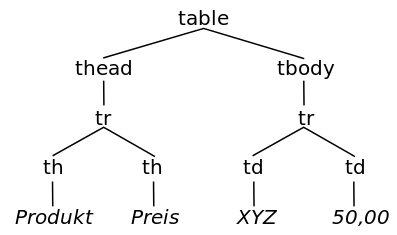
\includegraphics[width=0.5\textwidth]{abb/dom_sampletree}
  \caption[DOM Beispielbaum aus Listing \ref{lst:html5beispieltable}]{DOM Beispielbaum aus Listing \ref{lst:html5beispieltable}}
  \label{fig:dombeispielbaum}
\end{figure}

Selbstverständlich bietet das DOM die Möglichkeit der Modifizierung. So lassen sich Knoten nicht nur ändern, sondern auch entfernen und neu hinzufügen. Außerdem ist auf Grund der Baumstruktur ein Löschen eines Knotens möglich ohne die Integrität des Baumes zu zerstören.

\subsubsection{Ereignisse} Interaktive JavaScript Applikationen kommunizieren mit dem Browser über Events. Der Browser erzeugt für eine viel zahl von Nutzeraktionen Events, welche dann wiederum im Applikationscode abgefangen und verarbeitet werden können. In der DOM Level 0 Spezifikation werden Events lediglich an die Elemente verteilt an denen sie auftreten. Ist an diesem Element dann ein Event-Listener registriert wird dieser ausgeführt. DOM Level 2 hat die sogenannte Event-Propagation eingeführt. Diese Event Verteilung ist in drei Phasen aufgeteilt. Das Abfangen, dabei werden Events vom Document-Objekt den Dokumentbaum hinunter gereicht bis sie am Zielelement angelangt sind. Besitz ein Vorgänger Element im Dokumentbaum allerdings einen abfangenden Event-Listener wird auch dieser ausgelöst. Als nächstes wird löst das Event den Listener am Zielelement aus, was der DOM Level 0 Spezifikation gleicht. Die dritte Phase ist das sog. \textit{bubbling}. Hierbei steigt das Event wie ein Bläschen in der Dokument-Hierarchie zum Document-Objekt auf. Das Aufsteigen eines Events ist aber je nach Event unterschiedlich. Einige steigen auf andere nicht. Ein Event mit dem ein Formular beispielsweise abgeschickt wird muss nicht weiter im Dokumentbaum nach oben propagiert werden. Mausklick Events hingegen können für das gesamte Dokument sinnvoll verarbeitet werden und werden daher immer im Dokument aufsteigen.\\Ein Event-Listener kann auf drei unterschiedliche Arten an ein HTML Element gebunden werden. Eine Möglichkeit ist den Event-Listener direkt an das HTML Element mittels eines entsprechenden Event Attributs zu binden. So zu sehen in Zeile 1 in Listing \ref{lst:jseventhandler}. 

\vspace{1em}
\begin{lstlisting}[language=JavaScript, caption=JavaScript Event-Handler Beispiek, label=lst:jseventhandler]
<input type="button" name="b1" value="Drueck mich"
 onclick="alert('Button gedrueckt!');">

document.b1.onclick = function() { alert('Button gedrueckt!'); };

document.b1.addEventListener("click", click, false);
function click() { alert('Button gedrueckt!'); };
\end{lstlisting}

Da HTML statisch ist, ist auch der Event Listener in dem Fall statisch. Komplexe Applikationen verlangen aber eine dynamische Bindung von Listenern. Aus diesem Grund wurden mit dem DOM Level 2 zwei weitere Möglichkeiten einen Event-Listener zu registrieren standardisiert. So kann der Listener einerseits einfach einer Eigenschaft des DOM Objekts zugewiesen werden. Daraus resultiert ein klar strukturierter Code im HTML und JavaScript. Die Wartbarkeit wird außerdem verbessert. Andererseits lässt sich ein Listener über eine Objekt Methode binden. Diese Methode erwartet drei Argumente. Das erste bestimmt das Event auf welches der Listener reagieren soll. Das zweite Argument ist die Funktion die beim Eintreten des Events ausgeführt werden soll. Das dritte Argument, ein Boolescher Wert, legt fest ob der Event-Listener das Event nur abfängt wenn es direkt am Element oder dessen Kind Elementen auftritt. Dann muss dieser Wert \texttt{false} sein. Ansonsten kann der Event-Listener auch Events abfangen die im Geltungsbereich ihm über geordnet sind. Diese beiden Möglichkeit sind in Listing \ref{lst:jseventhandler} ab Zeile 4 zu sehen. Nachfolgend ist eine Übersicht einiger wichtiger Events.(vgl. \cite[S.428ff]{FlanJava2007})

\vspace{1em}
\begin{compactitem}
  \item onabort (bei Abbruch)
	\item onblur (beim Verlassen)
	\item onchange (bei erfolgter Änderung)
	\item onclick (beim Anklicken)
	\item ondblclick (bei doppeltem Anklicken)
	\item onerror (im Fehlerfall)
	\item onfocus (beim Aktivieren)
	\item onkeydown (bei gedrückter Taste)
	\item onkeypress (bei gedrückt gehaltener Taste)
	\item onkeyup (bei losgelassener Taste)
	\item onload (beim Laden einer Datei)
	\item onmousedown (bei gedrückter Maustaste)
	\item onmousemove (bei weiterbewegter Maus)
	\item onmouseout (beim Verlassen des Elements mit der Maus)
	\item onmouseover (beim Überfahren des Elements mit der Maus)
	\item onmouseup (bei losgelassener Maustaste)
	\item onreset (beim Zurücksetzen des Formulars)
	\item onselect (beim Selektieren von Text)
	\item onsubmit (beim Absenden des Formulars)
	\item onunload (beim Verlassen der Datei)
\end{compactitem}

\subsubsection{AJAX}
AJAX steht als Akronym für \textit{Asynchronous JavaScript and XML}. Geprägt wurde der Begriff AJAX von Jesse J. Garret.(vgl. \cite{JesseJGarret}) Es ist keine eigenständige Technologie, sondern vielmehr eine Bündelung einiger der verbreitetsten Web Technologien. Dazu gehört das HTTP Protokoll, JavaScript, XML und neuerdings auch JSON. Entwickelt wurde diese Technik von Microsoft, speziell von den Outlook Entwicklern. Diese benötigten eine Möglichkeit um HTTP Anfragen an einen Server abzusetzen ohne ein permanentes Neuladen der kompletten Webseite zu verursachen, um zu prüfen ob neue Mails vorhanden sind. Diese Anfragen sollten im Hintergrund ausgewertet und der entsprechende Teil der Webseite durch JavaScript, mit den nachgeladenen Informationen, verändert werden. Dadurch muss der Anwender nicht mit seiner Dateneingabe warten bis der Server mit der Auswertung der vorher eingegeben Daten fertig ist.\\Technisch erfolgt dies in drei Schritten. Zu erst wird ein AJAX Objekt erzeugt, dazu haben die Browser Hersteller das \texttt{XMLHttpRequest}-Objekt implementiert. Über dieses Objekt wird eine Verbindung zur Zielseite hergestellt. Als Parameter benötigt das Objekt die HTTP Übertragungsmethode, sprich \texttt{GET} oder \texttt{POST}. Außerdem die URL der Zielseite und zuletzt einen Booleschen Wert, der das Skript entweder synchron oder asynchron ausführen lässt. Zuletzt wird eine Rückgabefunktion angegeben die aufgerufen wird sobald der Server mit der Verarbeitung fertig ist und seine Antwort auf der Client Seite angekommen ist.(vgl. \cite[S.392ff]{WenzJava2008}) Abbildung \ref{fig:ajax} zeigt schematisch die Kommunikation zwischen Client und Server mit AJAX Technik. Bekanntestes Beispiel einer AJAX Implementation ist wohl der Vorschlag-Mechanismus der Google Suche.

\vspace{1em}
\begin{figure}[htb]
  \centering
  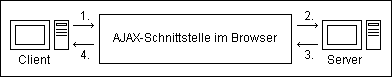
\includegraphics[width=1\textwidth]{abb/ajax_uml}
  \caption[AJAX Client/Server Kommunikation]{AJAX Client/Server Kommunikation \cite{ajax}}
  \label{fig:ajax}
\end{figure}

\subsubsection{jQuery}
jQuery ist die am meisten verbreitetste JavaScript Bibliothek im Internet. Mit 94,7\% Marktanteil, Stand 19.1.2015, ist jQuery klar der Marktführer bei den JavaScript Bibliotheken. Ganze 61,7\% der vom W3 Technology Survey analysierten Webseiten verwenden jQuery in ihrer Implementierung. (vgl. \cite{w3tech}) Die freie JavaScript Bibliothek jQuery stellt unter anderem umfangreiche Funktionen zur Manipulierung des DOM bereit. Daneben ist die Verwendung der AJAX Technik enorm vereinfacht worden von jQuery. Animationen und Effekte lassen sich schnell und unkompliziert mit der Bibliothek realsieren. Wie aus CSS bekannt verwendet jQuery Selektoren um auf die DOM Knoten zuzugreifen. Dank dem Programmierkonzept der \textit{fluent interfaces}, was soviel bedeutet wie sprechende Schnittstellen, kann ein erzeugtes jQuery Objekt sehr einfach an andere Funktionen weitergegeben werden.(vgl. \cite{wikijquery}) \glqq jQuery wird von \url{http://docs.jquery.com/} geladen und per Script-Tag in die HTML-Dokumente eingebunden.

\vspace{1em}
\begin{lstlisting}[language=HTML5, caption=jQuery Einbindung, label=lst:jqueryscript]
<script type="text/javascript"src="jquery.js"></script>
\end{lstlisting}

Die grundlegende Funktion von jQuery ist die Funktion jQuery() oder auch mit verringertem Schreibaufwand \$(), deren Verhalten abhängig ist von den jeweils gesetzten Parametern. Dabei fasst (sammelt) jede \$()-Funktion einen oder mehrere Knoten eines DOM-Baumes zusammen. In der einfachsten Form wird dann nur ein Ausdruck übergeben - meistens ein CSS-Selektor -, der alle passenden Elemente im Dokument findet.\grqq{}\cite{itwissenjquery}

\vspace{1em}
\begin{lstlisting}[language=JavaScript, caption=jQuery Selektor Syntax, label=lst:jqueryselektor]
$("selektor").funktionsname({ function({ }); });
\end{lstlisting}
	
Listing \ref{lst:jqueryselektor} zeigt die übliche Syntax einer jQuery Anweisung. Über den Selektor werden die Funktionen des erzeugten Objekts aufgerufen und eine entsprechende Rückgabe Funktion wird außerdem übergeben um auf das Ergebnis der Objekt Funktion reagieren zu können.

%\paragraph{Ereignisse}$\;$ \\
%// unterschiede zum JS Standard bei der Definierung, Einfachheit\\
%
%// Übersicht der wichtigsten Funktionen zu Events
%\vspace{1em}
%    \begin{compactitem}
%	    \item .bind – Handler an Event binden
%	    \item .on – Handler an Event binden
%	    \item .blur – Ereignis, wenn ein Element den Fokus verliert
%	    \item .click – Klick mit der Maustaste
%	    \item .dbclick – Doppelklick mit der Maustaste
%	    \item .hover – Mauszeiger bewegt sich über ein Element
%	    \item .mousemove – Mauszeiger bewegt sich in einem Element
%	    \item .keypress – eine Taste der Tastatur wird gedrückt
%	    \item .keyup – eine Taste der Tastatur wird losgelassen
%	    \item .change – ein Formularfeld wird verändert
%    \end{compactitem}
%    
%\paragraph{DOM-Manipulation}$\;$ \\
%// DOM Manipulation kurz anreißen\\

%\subsection{ABAP}
%// Herkunft/Entstehung\\
%// Grundlagen\\
%// Wichtige Elemente (OpenSQL)\\

\subsection{SAP UI5 Framework}
Kapitel 2.4 beschreibt das SAP UI 5 Framework der SAP AG. Beginnend wird mit einem kurzen Exkurs über die aktuelle UI Strategie der SAP AG, um zu verstehen wieso die SAP AG dieses Framework überhaupt entwickelt hat. Im Anschluss kommt eine allgemeine Definition, sowie die Beschreibung der verwendeten Softwarearchitektur. Zuletzt folgt eine kurze Erklärung des OData Protokolls und die Positionierung des Frameworks innerhalb einer SAP NetWeaver Landschaft.

\subsubsection{SAP UI Strategie}
Die SAP AG definiert ihre momentane \textit{User Experience} Strategie durch den Styleguide SAP Fiori und drei Schlagwörter -- \textit{New}, \textit{Renew} und \textit{Enable}. Unter \textit{New} wird verstanden, dass Entwicklern und Kunden neue Tools zur Entwicklung von SAP Applikationen und neue Applikationn selbst zur Verfügung gestellt werden. \textit{Renew} bedeutet, dass die vorhandenen Kernszenarios auf das neue UX portiert werden. SAP Screen Personas, auf das im Rahmen der Bachelorarbeit nicht weiter eingegangen wird, gehört zum Schlagwort \textit{Enable}. Kurz gesagt soll mit diesem Toolset das vorhandene UI der SAP Software an ein Unternehmen im Sinne des Corporate Design angepasst werden.(vgl. \cite{SAPUX})

\vspace{1em}
\begin{figure}[htb]
  \centering
  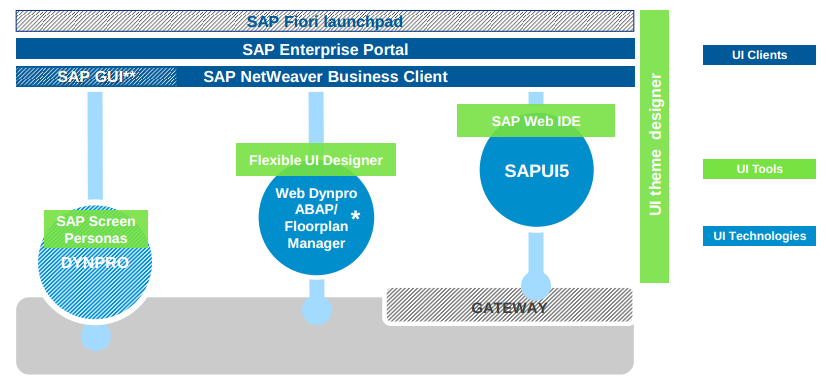
\includegraphics[width=0.9\textwidth]{abb/sap_key_ui_tools}
  \caption[SAP Schlüssel UI Tools und Technologien]{SAP Schlüssel UI Tools und Technologien \cite{SAPUXPDF}}
  \label{fig:sapkeyuitools}
\end{figure}

\subsubsection{Definition}
SAP UI5 ist ein SDK zur Entwicklung von Desktop- und mobilen Anwendungen die in einem Browser ausgeführt werden. Das Framework bündelt eine viel zahl an Technologien und Bibliotheken um den Entwicklungsprozess solcher Anwendungen bestmöglich zu unterstützen. Grundsätzlich basieren die, mit dem SDK entwickelten, Anwendungen auf den aktuellen Web-Entwicklungsstandards. Dazu gehören HTML 5, CSS 3 und JS. HTML 5 und CSS 3 werden, wie in den vorherigen Kapiteln geschildert, dafür verwendet um Struktur und Aussehen der Applikation zu gestalten. Bei JS hat man sich außerdem dazu entschieden zusätzlich die überaus populäre Erweiterungsbibliothek jQuery zu nutzen.(vgl. \cite{BuiltWith2014}) Das komplette SAP UI5 SDK ist freie Software und kann ohne jegliche SAP Lizenz bezogen und betrieben werden.

\subsubsection{Architektur}
\glqq Das Model-View-Controller-Architekturmuster strukturiert die Softwareentwicklung in die drei Einheiten: Datenmodell (Model), Präsentation (View) und Steuerung (Controller). Durch diese Trennung können die einzelnen Komponenten leichter erweitert, ausgetauscht oder wiederverwendet werden. Abbildung [... \ref{fig:mvcarch}] zeigt dieses Architekturmuster.
	
\vspace{1em}
\begin{figure}[htb]
  \centering
  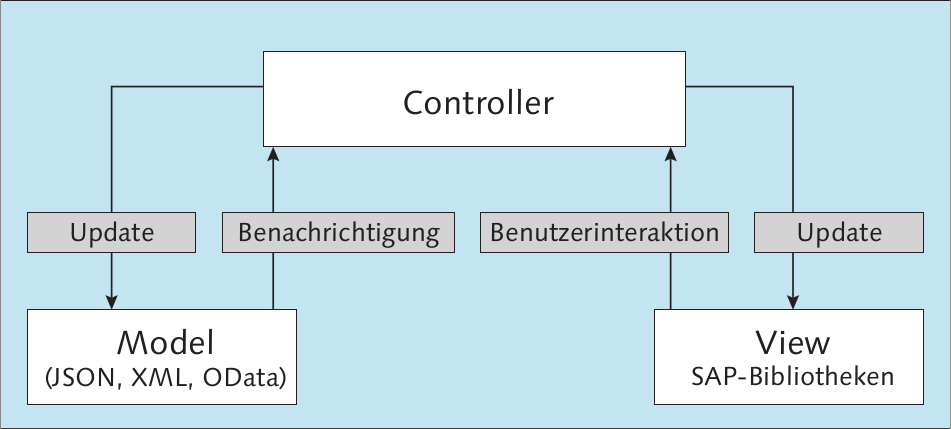
\includegraphics[width=0.7\linewidth]{abb/mvc_arch2}
  \caption[MVC-Architekturmuster]{MVC-Architekturmuster \cite[S.124]{AntoEinf2014}}
  \label{fig:mvcarch}
\end{figure}

Durch diese Trennung können z. B. zwei verschiedene Endgeräte das gleiche Model verwenden; der View wird z. B. einmal für die Desktop-Anwendung und einmal für das mobile Endgerät implementiert.\grqq{}\cite[S.123]{AntoEinf2014}

\paragraph{Model}$\;$ \\
Mit dem Model wird das Datenmodell abgebildet. Neben dem Datenbankzugriffsmechanismus stellt es die Applikationsdaten bereit und kann zudem auch die dazugehörige Geschäftslogik enthalten.

\paragraph{View}$\;$ \\
Benutzeraktionen werden vom View erfasst und zur weiteren Verarbeitung an den Controller weitergegeben. Damit fungiert das View als Präsentationsschicht zur visuellen Darstellung auf den verschiedenen Endgeräten.

\paragraph{Controller}$\;$ \\
Der Controller ist die zentrale Steuereinheit. Er nimmt Benutzeraktionen vom View entgegen und verarbeitet diese weiter. Ein Controller kann mehrere Views verwalten, zu jeder View gehört mindestens ein Controller. Bei Datenänderungen durch den Anwender koordiniert der Controller die Kommunikation mit dem Model.(vgl. \cite[S.123f]{AntoEinf2014})

\subsubsection{OData Protokoll}
\glqq Das Open Data Protocol (OData) ist ein von Microsoft veröffentlichtes Protokoll. Das Protokoll basiert auf HTTP und baut auf den älteren Protokollen ODBC und JDBC auf. OData ist primär für die sogenannten CRUD-Operationen, (Create, Read, Update und Delete) implementiert worden.\grqq{}\cite[S.168]{AntoEinf2014} Von der SAP AG ist der Einsatz der SAP NetWeaver Gateway Software vorgesehen, um einen entsprechenden OData Service im Backend bereit zustellen. Dadurch wird ein direkter Zugriff auf die dahinter liegenden Systeme verhindert. OData stellt eine API nach dem REST Prinzip bereit. Ein REST Service hat vier Eigenschaften die erfüllt sein müssen. Dazu gehört die Adressierbarkeit, jeder REST Service hat eine eindeutige Adresse den Uniform Resource Locator (URL). Der REST Server muss die angeforderten Daten in unterschiedlichen Formaten zurück geben können wie z.B HTML, JSON oder XML. Zustandslosigkeit ist eine weitere Eigenschaft. Sie besagt, dass weder der Server noch die Applikation Zustandsinformationen zwischen zwei Nachrichten speichert. Jede Anfrage an den Server ist in sich abgeschlossen. Die letzte Eigenschaft beschreibt die Operationen die ein REST Service bereitstellt. Bei einem Zugriff über HTTP werden die Methoden \texttt{GET}, \texttt{POST}, \texttt{PUT} und \texttt{DELETE} verwendeten um die CRUD Operationen zu ermöglichen.(vgl. \cite{wikirest})

\subsubsection{Positionierung im Netweaver Stack}
Eine mit SAP UI5 entwickelte Applikation wird als BSP Applikation auf dem SAP ABAP Application Server abgelegt. Von dort kann sie dann über die verschiedenen Endgeräte abgerufen werden. Aufgrund der verwendeten Technologien läuft die Anwendung weitestgehend auf dem jeweiligen Endgerät. Der ABAP AS dient lediglich dazu eingehende Anfragen, die vorher vom SAP NetWeaver Gateway entgegen genommen und weitergeleitet wurden, zu verarbeiten und eine entsprechende Antwort zurück zu schicken. Natürlich kann man auf das Gateway verzichtet, was aus Sicherheitsgründen jedoch nicht zu empfehlen ist. Auf Grund des verwendeten OData Protokolls und der REST Technik können problemlos Lastverteiler eingesetzt werden. Wodurch eine einfache Möglichkeit zur Skalierung geboten wird.(vgl. \cite{SAPFIORIARCH}) Abbildung \ref{fig:sapui5arch} zeigt eine schematische SAP Landschaft in der SAP UI5 integriert ist.

\vspace{1em}
\begin{figure}[htb]
  \centering
  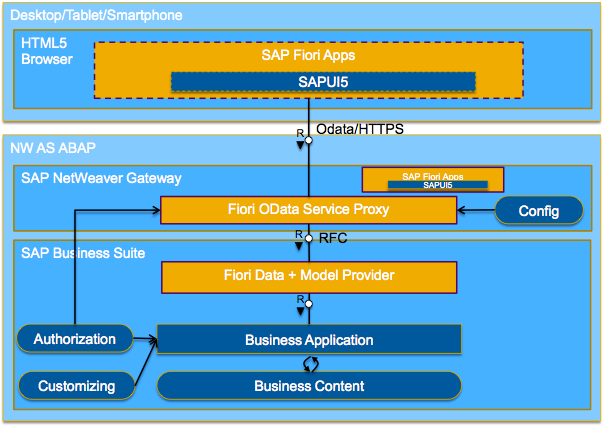
\includegraphics[width=0.8\linewidth]{abb/sap_ui5_architecture}
  \caption[Einordnung von SAP UI5 in die SAP System Landschaft]{Einordnung von SAP UI5 in die SAP System Landschaft \cite{SAPFIORIARCH}}
  \label{fig:sapui5arch}
\end{figure}

\newpage
\section{Fallbeispiel SAP UI5 Applikation}\label{fallbeispiel}
// Struktur des Kapitel

\subsection{Beschreibung}
// Frontend - Browser, Elemente\\
// Backend - JSON, OData Model\\
// Analyse der wichtigen Arbeitsschritte\\

\subsection{Hilfsmittel}
Dieses Kapitel soll kurz aufzeigen welche Hilfsmittel zur Realisierung des Prototypen verwendet wurden. Zum einen gehört die Entwicklungsumgebung Eclipse dazu. Weiter wurden die Chrome Developer Tools des Chrome Browser genutzt, sowie das Tool Wireframesketcher. In den folgenden Unterkapitel werden diese Tools kurz vorgestellt.

\subsubsection{Eclipse}
Zum Einsatz in der Implementierung des Fallbeispiels ist die quelloffene integrierte Entwicklungsumgebung Eclipse gekommen. Diese IDE wurde von der Eclipse Foundation entwickelt und ist plattformunabhängig. Geschrieben wurde Eclipse in Java. Die aktuelle Version 4.4 ist am 25. Juni 2014 erschienen und trägt den Namen Luna. Eclipse zeichnet sich durch ein Plugin System aus mit welchem eine erhebliche Anzahl an Anwendungsfälle mit dieser IDE abgedeckt werden können.(vgl. \cite{WikiEclipse2014}) So auch die Entwicklung von SAP UI5 Applikationen. Dafür hat die SAP AG ein spezielles SAP UI5 Plugin bereitgestellt. Entsprechende Plugins müssen nicht umständlich über eine Webseite bezogen und installiert werden. Sie können über die integrierte Plugin Funktion installiert und eingerichtet werden. Eine URL zum Plugin ist vollkommen ausreichend. Für die Entwicklung von SAP UI5 Applikationen wurden folgende Plugins benötigt:
	
	\vspace{1em}
    \begin{compactitem}
	    \item UI Development Toolkit for HTML5
	    \item ABAP Development Tools for SAP NetWeaver
	    \item (SAP HANA Tools)	    
    \end{compactitem}

Bezogen werden können diese Plugins mittels der URL \url{https://tools.hana.ondemand.com/luna} und der erwähnten Plugin Funktion von Eclipse. Neben dem reinen Code Editor werden allerdings weitere Tools benötigt um eine SAP UI5 Applikation zu entwickeln.

\subsubsection{Chrome Developer Tools}
Die SAP UI5 Dokumentation schlägt vor zum Testen der entwickelten Applikationen Google Chrome oder Mozilla Firefox anstatt Microsoft Internet Explorer zu verwenden. Das vorliegende Fallbeispiel wurde mit Google Chrome getestet. Google Chrome bietet dazu ein Tool mit dem Namen Developer Tools, welches in jeder Standard Installation des Browsers enthalten ist. Mit diesem Tool lässt sich beispielsweise das DOM der aktuellen Webseite anzeigen. Weiter kann man JavaScript Breakpoints setzen und so effizient debuggen. Es bietet eine Konsole um direkte JavaScript Befehle abzusetzen und die Ergebnisse zu analysieren. Um eine Anwendungen nicht zwingend auf verschiedenen Endgeräten, mit verschiedenen Displaygrößen, testen zu müssen lassen sich jegliche Art von Endgeräten mit den Developer Tools emulieren.(vgl. \cite{DevTools})

%\subsubsection{Neptune Application Designer}

\subsubsection{Wireframesketcher}
// Wireframing als Prototyping\\
// Abbildung Wireframesketcher\\

\subsection{Implementierung}
// Struktur des Kapitel

\subsubsection{View}
// Auszugsweise Coding bringen um bestimmte Elemente aus der Theorie zu zeigen\\
// Generellen Aufbau der Views erklären\\
// Kapselung wird dadurch verdeutlicht\\
// Bootstrapping der Applikation\\
// Listing \ref{lst:app.view.js}
	\vspace{1em}
	\begin{lstlisting}[frame=htrbl, caption=Root View der Applikation, label=lst:app.view.js]
sap.ui.jsview("abat.Mockup.view.App", {

  getControllerName: function () {
    return "abat.Mockup.view.App";
  },
  
  createContent: function (oController) {
    // to avoid scroll bars on desktop
    this.setDisplayBlock(true);
    
    // create app
    this.app = new sap.m.SplitApp();
    
    // load the master page
    var master = sap.ui.xmlview("Master", "abat.Mockup.view.Master");
    master.getController().nav = this.getController();
    this.app.addPage(master, true);
    
    // load the empty page
    var empty = sap.ui.xmlview("Empty", "abat.Mockup.view.Empty");
    this.app.addPage(empty, false);
    
    // wrap app with shell
    return new sap.m.Shell("Shell", {
      title : "{i18n>ShellTitle}",
      showLogout : false,
      app : this.app
    });
  }
});
	\end{lstlisting}

// Master/Detail Applikation mit Fragment und Chart View Aufbau\\
// TODO: Visio Diagramm oder vergleichbares erstellen\\
// sap.ui.view\\
//   |- sap.m.Shell\\
//   |  |- sap.m.SplitApp\\
//   |  |  |- sap.m.Page\\
//   |  |  |  |- sap.m.Bar\\
//   |  |  |  |- sap.m.Bar\\
//   |  |  |  |- sap.m.List\\
//   |  |  |  |  |- sap.m.ObjectListItem\\
//   |  |  |  |- sap.m.Bar\\
//   |  |  |- sap.m.Page\\
//   |  |  |  |- sap.m.ObjectHeader\\
//   |  |  |  |  |- sap.m.ObjectAttribute\\
//   |  |  |  |  |- sap.m.ObjectAttribute\\
//   |  |  |  |  |- sap.m.ObjectAttribute\\
//   |  |  |  |  |- sap.m.ObjectAttribute\\
//   |  |  |  |  |- sap.m.ObjectStatus\\
//   |  |  |  |- sap.IconTabBar\\
//   |  |  |  |  |- sap.IconTabFilter\\
//   |  |  |  |  |  |- sap.ui.core.Fragment\\
//   |  |  |  |  |  |  |- sap.ui.core.FragmentDefinition\\
//   |  |  |  |  |  |  |  |- sap.viz.ui5.Bar\\
//   |  |  |  |  |- sap.IconTabFilter\\
//   |  |  |  |  |  |- sap.ui.core.Fragment\\
//   |  |  |  |  |  |  |- sap.ui.core.FragmentDefinition\\
//   |  |  |  |  |  |  |  |- sap.viz.ui5.Bar\\
//   |  |  |  |- sap.m.Bar\\

\subsubsection{Model und Controller}
// die Verbindung von beiden Anhand von Coding zeigen\\
// TODO: OData Modell einbinden\\
// Datenfluss anreißen und auf Analyse verweisen\\
// Listing \ref{lst:Component.js}
	\vspace{1em}
	\begin{lstlisting}[frame=htrbl, caption=Component.js - Datenmodell an die Root View binden, label=lst:Component.js]
...
// JSON Modell an die Root View binden
var oModel = new sap.ui.model.json.JSONModel("model/mock.json");
oView.setModel(oModel);

// OData Modell
var oModel = new sap.ui.model.odata.ODataModel(<URL>);
oView.setModel(oModel);

// I18N(Lokalisierung) Modell
var i18nModel = new sap.ui.model.resource.ResourceModel({
  bundleUrl : "i18n/messageBundle.properties"
});
oView.setModel(i18nModel, "i18n");

// Geraetespezifisches Modell
var deviceModel = new sap.ui.model.json.JSONModel({
  isPhone : jQuery.device.is.phone,
  listMode : (jQuery.device.is.phone) ? "None" : "SingleSelectMaster",
  listItemType : (jQuery.device.is.phone) ? "Active" : "Inactive"
});
deviceModel.setDefaultBindingMode("OneWay");
oView.setModel(deviceModel, "device");
...
	\end{lstlisting}

\subsubsection{Backend}
// ABAP Stack der den RESTful Service bereitstellt zeigen\\
// Beispielhafte Implementation des HTTP Responses\\

\newpage
\section{Objektorientierte Analyse}\label{analyse}
Im Kapitel Objektorientierte Analyse wird der Prototyp und das verwendete SAP UI5-Framework analysiert so wie die Ergebnisse in Form von Diagrammen gezeigt und beschrieben. Anfangs werden die Kombinationsmöglichkeiten zwischen den einzelnen Bibliotheken des SAP UI5-Frameworks aufgezeigt. Im Anschluss folgt eine Verdeutlichung des Nachrichtenflusses innerhalb der SAP UI5-Applikation.

\subsection{Bibliotheken Beziehungen}
Im Zuge der Analyse des SAP UI5-Frameworks wurde zuerst offengelegt, wie die einzelnen Bibliotheken, innerhalb des Frameworks, miteinander kombinierbar sind. Dadurch konnte festgestellt werden, dass einige Bibliotheken zu Gruppen zusammen gefasst werden können und zwei Bibliotheken außenvor liegen. Das wäre zum einen die Bibliothek \texttt{sap.viz}. Mit ihr wird eine Charting-Bibliothek bereitgestellt, die sich mit allen anderen Bibliotheken verwenden lässt. Und zum anderen die Bibliothek \texttt{sap.ui.inbox}, welche eine fertige Inbox darstellt, um sie in Applikationen einzubinden. Die Bibliotheken \texttt{sap.ui.core}, \texttt{sap.ui.layout} und \texttt{sap.ui.unified} lassen sich klar als Kernbibliotheken einordnen. Sie stellen das Grundgerüst des Frameworks dar. Dann gibt es noch eine Gruppe von Bibliotheken die Controls bereitstellen, die an die Bedürfnisse einer Desktop-Applikation geknüpft sind. Die letzte Gruppe beinhaltet Bibliotheken für Mobile-Controls. Sämtliche Mobile-Controls funktionieren auch in einer Desktop-Applikation. Sie sind jedoch für die Anzeige auf mobilen Endgeräten optimiert. Mit Abbildung \ref{fig:sapui5libconnections} werden diese Gruppen und Beziehungen dargestellt.

\vspace{1em}
\begin{figure}[htb]
  \centering
  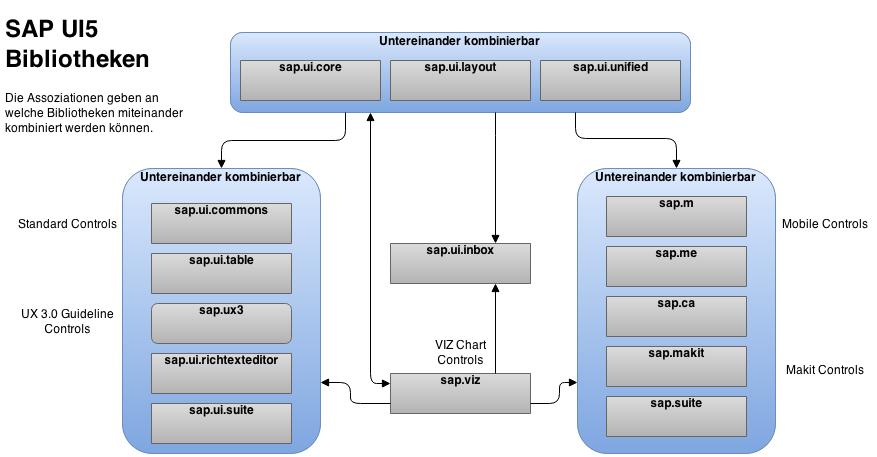
\includegraphics[width=0.95\linewidth]{abb/sapui5_lib_connections}
  \caption[Klassendiagramm: SAP UI5-Bibliotheken Kombinationen]{Klassendiagramm: SAP UI5-Bibliotheken Kombinationen}
  \label{fig:sapui5libconnections}
\end{figure}

\newpage
\subsection{Modularität}
Durch die stringente Verwendung des MVC-Musters können Templates entwickelt werden. Mit diesen Templates lassen sich beispielsweise komplette Geschäftsprozesse abbilden. Geschäftslogik und Präsentation leben in ihrem eigenen Model-View-Controller Verbund. Dadurch kann man sie in den verschiedensten Applikationen wiederverwenden. Der Wartungsaufwand für eine komplexe Applikation lässt sich so verringern. Neben dem MVC-Muster kommt eine zusätzliche Trennung der Präsentationsschicht zum Tragen. Die Struktur wird in JavaScript oder XML definiert, wohingegen die Optik mit CSS beschrieben wird. Dadurch können die Templates schnell und ohne große Hindernisse an ein Corporate Design angepasst werden. Abbildung \ref{fig:sapui5mvctemplates} zeigt diesen denkbaren Einsatz von fertigen UI Templates.

\vspace{1em}
\begin{figure}[htb]
  \centering
  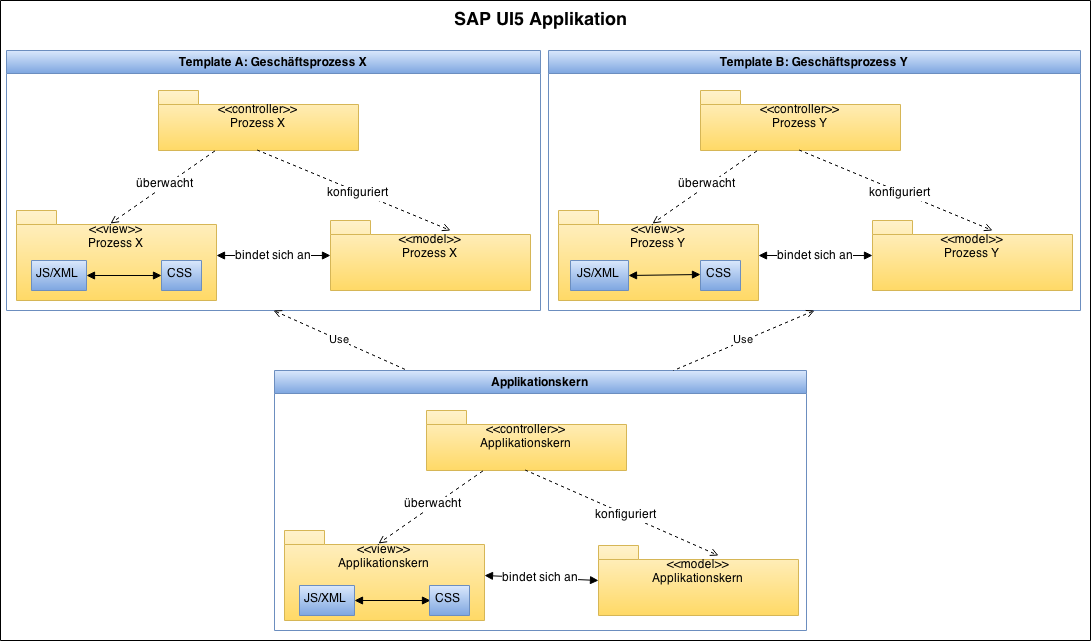
\includegraphics[width=1\linewidth,angle=90]{abb/sapui5_mvc_templates}
  \caption[Paketdiagramm: MVC-Templates innerhalb einer SAP UI5-Applikation]{Paketdiagramm: MVC-Templates innerhalb einer SAP UI5-Applikation}
  \label{fig:sapui5mvctemplates}
\end{figure}

\newpage
\subsection{User Interface Kaskade}
Um ein besseres Verständnis der UI-Aufruffolge zu erhalten, wurde ein Sequenzdiagramm angefertigt. Mit diesem Diagramm wurde der Aufruf eines Listeneintrags auf der Hauptseite abgebildet. Dieser Klick verursacht die Applikation dazu die ID und den Datenkontext des Eintrags über den Controller an die Detailseite weiterzugeben und dort die vorhandenen Informationen darzustellen. Auf dem Weg dorthin übernimmt der Controller der Detailseite die Aufgabe die beiden verfügbaren Charts zu konfigurieren. Dabei werden die Beschriftung und die Datenherkunft festgelegt.

\vspace{1em}
\begin{figure}[htb]
  \centering
  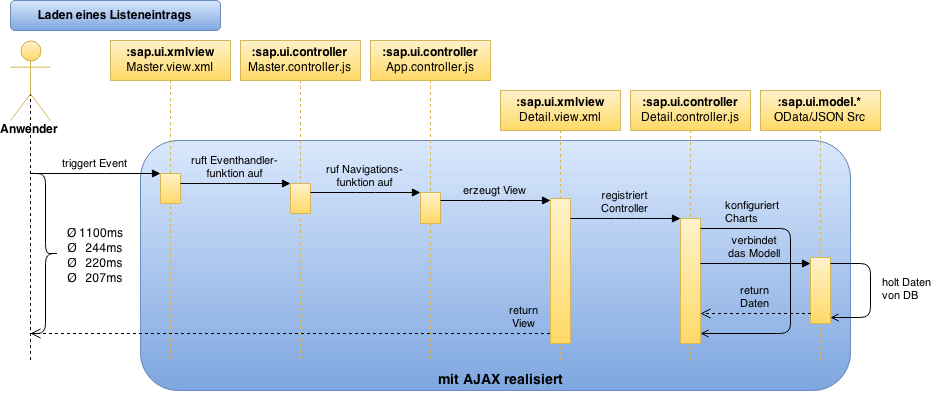
\includegraphics[width=1.1\linewidth,angle=90]{abb/sapui5_load_list_entry}
  \caption[Sequenzdiagramm: Laden eines Listeneintrags]{Sequenzdiagramm: Laden eines Listeneintrags}
  \label{fig:sapui5loadlistentry}
\end{figure}

\paragraph{Zeitmessung}$\;$ \\
Um das Sequenzdiagramm mit Meta-Informationen anzureichern, wurde eine Zeitmessung vorgenommen. Dazu wurden die Chrome-Developer-Tools benutzt. Es wurden vier Werte gemessen. Alle Versuche wurden mit deaktiviertem Browser-Cache gemessen. Die erste Messgröße ist die Dauer vom Öffnen bis zur fertig geladenen Seite. Danach wurden drei Einträge aus der Liste gewählt und jeweils gewartet, bis die Detailseite vollständig geladen und das Chart aufgebaut war. Aus den erhobenen Versuchswerten ist noch der arithmetische Durchschnitt gebildet worden. Alle Ergebnisse sind in Tabelle \ref{tab:uiloading} aufgeführt.

\vspace{1em}
\begin{center}
  \begin{tabular}{ | c | c | c | c | c | c | }
  \hline
  \textbf{Versuch}
  & \textbf{Seite} & \textbf{Detail} & \textbf{1. Klick} & \textbf{2. Klick} & \textbf{3. Klick}\\
  \hline \hline
  1 & 756ms & 742ms & 382ms & 227ms & 205ms\\
  \hline
  2 & 804ms & 877ms & 515ms & 214ms & 205ms\\
  \hline
  3 & 691ms & 888ms & 390ms & 219ms & 200ms\\
  \hline
  4 & 774ms & 743ms & 384ms & 229ms & 200ms\\
  \hline
  5 & 696ms & 736ms & 387ms & 282ms & 206ms\\
  \hline
  6 & 727ms & 818ms & 382ms & 215ms & 211ms\\
  \hline
  7 & 882ms & 620ms & 378ms & 221ms & 281ms\\
  \hline
  8 & 748ms & 729ms & 391ms & 299ms & 210ms\\
  \hline
  9 & 698ms & 729ms & 383ms & 241ms & 276ms\\
  \hline
  10 & 684ms & 881ms & 389ms & 213ms & 198ms\\
  \hline \hline
  \textbf{\O} & \textbf{746ms} & \textbf{776ms} & \textbf{398ms} & \textbf{236ms} & \textbf{199ms}\\
  \hline
  \end{tabular}
\captionof{table}{Chrome Browser UI Ladezeiten}
\label{tab:uiloading}
\end{center}

Aus diesen Ergebnissen lässt sich ablesen, dass das UI beim ersten Aufruf der Applikation im Durchschnitt in unter einer Sekunde geladen und für den Anwender sichtbar ist. Dabei ist zu sagen, dass sich die Ergebnisse der selben Versuchsreihe, mit aktiviertem Browser-Cache, nur minimal zu den Ergebnissen mit deaktiviertem Browser-Cache unterscheiden. Erfolgt dann der Klick vom Anwender auf einen Listeneintrag wird von der Applikation die Detailseite geladen. Dies geschieht durchschnittlich in 776 Millisekunden. Bei der Auswahl eines ersten Listeneintrags, ganz gleich seiner Position innerhalb der Liste, dauert das Laden der Informationen innerhalb der Detailseite im Durchschnitt 398 Millisekunden. Das Laden der Daten und das Aktualisieren der Detailseite dauerten beim zweiten und dritten Listeneintrag im Durchschnitt 236 und 199 Millisekunden. Diese Zahlen zeigen, dass sich eine Applikation, die mit den SAP UI5-Bibliotheken entwickelt wurde, zumindest bei niedriger Komplexität genauso performant in der Präsentation behauptet, wie eine Standard SAP GUI-Transaktion.


\newpage
\section{Fazit}\label{fazit}
Lorem ipsum dolor sit amet.

\paragraph{Zusammenfassung}
// Arbeitsgebiete, Produktions \& Dienstleistungsbereiche\\
// Arbeitsergebnisse\\
// Projektziele, Projektergebnisse, Projekttermine\\
// Mitwirkungszeiträume\\
// Liste aller selbst wahrgenommen Aufgaben und Tätigkeiten\\
// Projektmeilensteine\\
// Ablauforganisation \& Beteiligte\\
// Arbeitsformen, Arbeitsmittel, Arbeitsabläufe\\
// Kommunikations- / Informationsgewohnheiten\\
// Auswertung relevanter Literatur\\
// Themen aus Lehrveranstaltungen\\

\paragraph{Bewertung}
// Wesentliche Erkenntnisse und Erfahrungen\\
// Folgerungen und Konsequenzen\\
// Vorschläge für Verbesserung und Veränderung\\
// Auswirkungen auf persönliche Berufs- und Karriereplanung\\
// Bezug zum Studium\\
// hilfreiche Studieninhalte\\
// neu gewonnenes Interesse\\

% einfacher Zeilenabstand
\onecolumn
\singlespacing

% das Literaturverzeichnis
\newpage

% römische Numerierung wieder setzen
\pagenumbering{Roman}
\setcounter{page}{6}
\addcontentsline{toc}{section}{Literaturverzeichnis}
\renewcommand\refname{Literaturverzeichnis}
\bibliography{Literatur}

%% Index soll Stichwortverzeichnis heissen
% \newpage
% % Stichwortverzeichnis soll im Inhaltsverzeichnis auftauchen
% \addcontentsline{toc}{section}{Stichwortverzeichnis}
% \renewcommand{\indexname}{Stichwortverzeichnis}
% % Stichwortverzeichnis endgueltig anzeigen
% \printindex

% der Anhang
\onehalfspacing
\newpage
\addcontentsline{toc}{section}{Anhang}
\fancyhead[L]{Anhang}
\subsection*{Anhang}\label{anhang}
\subsubsection*{index.html}
\begin{lstlisting}[frame=htrbl, label=lst:index.html]
<!DOCTYPE html>
<html>
<head>
<meta http-equiv="X-UA-Compatible" content="IE=edge" />
<meta http-equiv='Content-Type' content='text/html;charset=UTF-8' />

<title>abat AG - Mockup Claas</title>

<script id="sap-ui-bootstrap" src="resources/sap-ui-core.js"
	data-sap-ui-theme="sap_bluecrystal"
	data-sap-ui-libs="sap.m, sap.ui.layout"
	data-sap-ui-preload=""
	data-sap-ui-xx-bindingSyntax="complex"
	data-sap-ui-resourceroots='{
				"abat.Mockup": "./"
			}'>
</script>

<script>
  new sap.ui.core.ComponentContainer({
    name : "abat.Mockup"
  }).placeAt("content");
</script>

</head>
<body class="sapUiBody" role="application">
	<div id="content"></div>
</body>
</html>
\end{lstlisting}

\newpage
\subsubsection*{Component.js}
\begin{lstlisting}[frame=htrbl, label=lst:Component.js]
jQuery.sap.declare("abat.Mockup.Component");

sap.ui.core.UIComponent.extend("abat.Mockup.Component", {

  createContent : function() {

    // create root view
    var oView = sap.ui.view({
      id : "app",
      viewName : "abat.Mockup.view.App",
      type : "JS",
      viewData : {
        component : this
      }
    });

    // set data model on root view
    var oModel = new sap.ui.model.json.JSONModel("model/mock.json");
    oView.setModel(oModel);

    // set i18n model
    var i18nModel = new sap.ui.model.resource.ResourceModel({
      bundleUrl : "i18n/messageBundle.properties"
    });
    oView.setModel(i18nModel, "i18n");

    // set device model
    var deviceModel = new sap.ui.model.json.JSONModel({
      isPhone : jQuery.device.is.phone,
      listMode : (jQuery.device.is.phone) ? "None" : "SingleSelectMaster",
      listItemType : (jQuery.device.is.phone) ? "Active" : "Inactive"
    });
    deviceModel.setDefaultBindingMode("OneWay");
    oView.setModel(deviceModel, "device");

    // done
    return oView;
  }
});
\end{lstlisting}

\newpage
\subsubsection*{App.view.js}
\begin{lstlisting}[frame=htrbl, label=lst:App.view.js]
sap.ui.jsview("abat.Mockup.view.App", {

  getControllerName : function() {
    return "abat.Mockup.view.App";
  },

  createContent : function(oController) {

    // to avoid scroll bars on desktop the root view must be set to block
    // display
    this.setDisplayBlock(true);

    // create app
    this.app = new sap.m.SplitApp();

    // load the master page
    var master = sap.ui.xmlview("Master", "abat.Mockup.view.Master");
    master.getController().nav = this.getController();
    this.app.addPage(master, true);

    // load the empty page
    var empty = sap.ui.xmlview("Empty", "abat.Mockup.view.Empty");
    this.app.addPage(empty, false);

    // wrap app with shell
    return new sap.m.Shell("Shell", {
      title : "{i18n>ShellTitle}",
      showLogout : false,
      app : this.app
    });
  }
});
\end{lstlisting}

\newpage
\subsubsection*{App.controller.js}
\begin{lstlisting}[frame=htrbl, label=lst:App.controller.js]
sap.ui.controller("abat.Mockup.view.App", {

  /**
   * Navigates to another page
   * 
   * @param {string} pageId The id of the next page
   * @param {sap.ui.model.Context} context The data context
   */
  to : function(pageId, context) {

    var app = this.getView().app;

    // load page on demand
    var master = ("Master" === pageId);
    if (app.getPage(pageId, master) === null) {
      var page = sap.ui.view({
        id : pageId,
        viewName : "abat.Mockup.view." + pageId,
        type : "XML"
      });
      page.getController().nav = this;
      app.addPage(page, master);
      jQuery.sap.log.info("app controller > loaded page: " + pageId);
    }

    // show the page
    app.to(pageId);

    // set data context on the page
    if (context) {
      var page = app.getPage(pageId);
      page.setBindingContext(context);
    }
  },

  /**
   * Navigates back to a previous page
   * 
   * @param {string} pageId The id of the next page
   */
  back : function(pageId) {
    this.getView().app.backToPage(pageId);
  }
});
\end{lstlisting}

\newpage
\subsubsection*{Master.view.xml}
\begin{lstlisting}[frame=htrbl, label=lst:Master.view.xml]
<core:View controllerName="abat.Mockup.view.Master" xmlns="sap.m"
  xmlns:core="sap.ui.core">
  <Page>
    <customHeader>
      <Bar>
        <contentLeft>
          <Image src="img/logo.png" width="173px" height="30px"></Image>
        </contentLeft>
      </Bar>
    </customHeader>
    <subHeader>
      <Bar>
        <contentLeft>
          <SearchField search="handleSearch" width="100%">
          </SearchField>
        </contentLeft>
      </Bar>
    </subHeader>
    <List id="list" mode="{device>/listMode}" select="handleListSelect"
      items="{/Products}">
      <ObjectListItem type="{device>/listItemType}"
        press="handleListItemPress"
        title="{MaterialName}"
        number="{Quantity}"
        numberUnit="{i18n&gt;QuantityUnit}"
        numberState="{parts : [ 'Quantity', 'MinimalQuantity' ],
          formatter : 'abat.Mockup.util.Formatter.numberState'}">
        <attributes>
          <ObjectAttribute text="{MatId}" />
        </attributes>
        <firstStatus>
          <ObjectStatus text="{Status}"
            state="{path: 'Status',
              formatter: 'abat.Mockup.util.Formatter.statusState'}" />
        </firstStatus>
      </ObjectListItem>
    </List>
    <footer>
      <Bar>
        <contentRight>
          <Button icon="sap-icon://group-2" press="handleViewSettings" />
        </contentRight>
      </Bar>
    </footer>
  </Page>
</core:View>
\end{lstlisting}

\newpage
\subsubsection*{Master.controller.js}
\begin{lstlisting}[frame=htrbl, label=lst:Master.controller.js]
jQuery.sap.require("abat.Mockup.util.Formatter");
jQuery.sap.require("abat.Mockup.util.Grouper");

sap.ui.controller("abat.Mockup.view.Master", {

  onExit : function() {
    if (this._lineItemViewDialog) {
      this._lineItemViewDialog.destroy();
      this._lineItemViewDialog = null;
    }
  },

  handleListItemPress : function(evt) {
    var context = evt.getSource().getBindingContext();
    this.nav.to("Detail", context);
  },

  handleSearch : function(evt) {
    // create model filter
    var filters = [];
    var query = evt.getParameter("query");
    if (query && query.length > 0) {
      var filter = new sap.ui.model.Filter("MaterialName",
          sap.ui.model.FilterOperator.Contains, query);
      filters.push(filter);
    }

    // update list binding
    var list = this.getView().byId("list");
    var binding = list.getBinding("items");
    binding.filter(filters);
  },

  handleListSelect : function(evt) {
    // get binding context and nav to detail page
    var context = evt.getParameter("listItem").getBindingContext();
    this.nav.to("Detail", context);
  },

  handleViewSettings : function(evt) {
    var that = this;
    if (!this._lineItemViewDialog) {
      // create dialog
      this._lineItemViewDialog = new sap.m.ViewSettingsDialog({
        groupItems : [ new sap.m.ViewSettingsItem({
          text : "Price",
          key : "GrossAmount"
        }), new sap.m.ViewSettingsItem({
          text : "Status",
          key : "Status"
        }) ],
        confirm : function(evt) {
          var aSorters = [];
          var mParams = evt.getParameters();
          if (mParams.groupItem) {
            var sPath = mParams.groupItem.getKey();
            var bDescending = mParams.groupDescending;
            var vGroup = abat.Mockup.util.Grouper[sPath];
            aSorters.push(
              new sap.ui.model.Sorter(sPath, bDescending, vGroup));
          }
          var oBinding = that.getView().byId("list").getBinding("items");
          oBinding.sort(aSorters);
        }
      });
    }

    // open dialog
    this._lineItemViewDialog.open();
  }
});
\end{lstlisting}

\newpage
\subsubsection*{Detail.view.xml}
\begin{lstlisting}[frame=htrbl, label=lst:Detail.view.xml]
<core:View controllerName="abat.Mockup.view.Detail" xmlns="sap.m"
  xmlns:core="sap.ui.core">
  <Page title="{i18n>DetailTitle}"
    class="sapUiFioriObjectPage"
    showNavButton="{device>/isPhone}" 
    navButtonPress="handleNavButtonPress">
    <ObjectHeader title="{MaterialName}" number="{Quantity}"
      numberUnit="{i18n&gt;QuantityUnit}"
      numberState="{parts: [ 'Quantity', 'MinimalQuantity' ],
        formatter: 'abat.Mockup.util.Formatter.numberState'}"
      icon="img/placeholder.gif">
      <attributes>
        <ObjectAttribute 
          text="{i18n&gt;MatId}: {MatId}" />
        <ObjectAttribute
          text="{i18n&gt;GrossAmount}: {GrossAmount} {CurrencyCode}" />
        <ObjectAttribute
          text="{i18n&gt;TaxAmount}: {TaxAmount} {CurrencyCode}" />
        <ObjectAttribute
          text="{i18n&gt;NetAmount}: {NetAmount} {CurrencyCode}" />
      </attributes>
      <firstStatus>
        <ObjectStatus text="{Status}"
          state="{path: 'Status',
                  formatter: 'abat.Mockup.util.Formatter.statusState'}" />
      </firstStatus>
    </ObjectHeader>
    <IconTabBar expanded="{device>/isNoPhone}">
      <items>
        <IconTabFilter text="{i18n&gt;IconTab_1}"
          icon="sap-icon://vertical-bar-chart-2">
          <content>
            <core:Fragment type="XML"
              fragmentName="abat.Mockup.view.ForecastChart"></core:Fragment>
          </content>
        </IconTabFilter>
        <IconTabFilter text="{i18n&gt;IconTab_2}" icon="sap-icon://line-chart">
          <content>
            <core:Fragment type="XML"
              fragmentName="abat.Mockup.view.OrderProposalChart"></core:Fragment>
          </content>
        </IconTabFilter>
      </items>
    </IconTabBar>
    <footer>
      <Bar>
        <contentRight>
          <Button text="{i18n>ApproveButtonText}" icon="sap-icon://accept"
            press="handleApprove" />
        </contentRight>
      </Bar>
    </footer>
  </Page>
</core:View>
\end{lstlisting}

\newpage
\subsubsection*{Detail.controller.js}
\begin{lstlisting}[frame=htrbl, label=lst:Detail.controller.js]
jQuery.sap.require("abat.Mockup.util.Formatter");
jQuery.sap.require("sap.m.MessageBox");
jQuery.sap.require("sap.m.MessageToast");

sap.ui.controller("abat.Mockup.view.Detail", {

  onInit : function(evt) {
    this.configForecastChart();
    this.configOrderProposalChart();
  },

  handleForecastDataSelect : function(evt) {
    var xAxisIndex = (evt.getParameter("data")[0]).data[0].ctx.path.dii_a1;
    var oContext = this.getView().byId("lineChart").getBindingContext();
    var oSelectedData = this.getView().getModel().getProperty(
        oContext.sPath + "/ForecastData/" + xAxisIndex);

    console.log(oSelectedData);
  },

  handleOrderProposalDataSelect : function(evt) {
    // TODO write code to make Chart dynamic
  },

  handleNavButtonPress : function(evt) {
    this.nav.back("Master");
  },

  handleApprove : function(evt) {
    // show confirmation dialog
    var bundle = this.getView().getModel("i18n").getResourceBundle();
    sap.m.MessageBox.confirm(bundle.getText("ApproveDialogMsg"), function(
        oAction) {
      if (sap.m.MessageBox.Action.OK === oAction) {
        // notify user
        var successMsg = bundle.getText("ApproveDialogSuccessMsg");
        sap.m.MessageToast.show(successMsg);
        // TODO call proper service method and update model
      }
    },

    bundle.getText("ApproveDialogTitle"));
  },

  configForecastChart : function() {
    var oDatasetForecast = new sap.viz.ui5.data.FlattenedDataset({
      dimensions : [ {
        axis : 1,
        name : 'Month',
        value : "{Month}"
      } ],
      measures : [ {
        name : 'Menge1',
        value : '{Menge1}'
      }, {
        name : 'Menge2',
        value : '{Menge2}'
      } ],
      data : {
        path : "ForecastData"
      }
    });

    oLineChart = this.getView().byId("lineChart");
    oLineChart.setTitle(new sap.viz.ui5.types.Title({
      visible : true,
      text : "{i18n>ForecastChartTitle}"
    }));
    oLineChart.setDataset(oDatasetForecast);
  },

  configOrderProposalChart : function() {
    var oDatasetOrderProposal = new sap.viz.ui5.data.FlattenedDataset({
      dimensions : [ {
        axis : 1,
        name : 'Month',
        value : "{Month}"
      } ],
      measures : [ {
        name : 'Menge1',
        value : '{Menge1}'
      } ],
      data : {
        path : "OrderProposalData"
      }
    });

    oBarChart = this.getView().byId("barChart");
    oBarChart.setTitle(new sap.viz.ui5.types.Title({
      visible : true,
      text : "{i18n>OrderProposalChartTitle}"
    }));
    oBarChart.setDataset(oDatasetOrderProposal);
  }
});
\end{lstlisting}

\newpage
\subsubsection*{ForecastChart.fragment.xml}
\begin{lstlisting}[frame=htrbl, label=lst:ForecastChart.fragment.xml]
<core:FragmentDefinition xmlns:core="sap.ui.core"
  xmlns:mvc="sap.ui.core.mvc" 
  xmlns="sap.m" 
  xmlns:html="http://www.w3.org/1999/xhtml"
  xmlns:viz="sap.viz.ui5" 
  xmlns:types="sap.viz.ui5.types">
  <viz:Line id="lineChart" width="100%" height="400px"
    selectData="handleForecastDataSelect"></viz:Line>
</core:FragmentDefinition>
\end{lstlisting}

\subsubsection*{OrderProposalChart.fragment.xml}
\begin{lstlisting}[frame=htrbl, label=OrderProposalChart.fragment.xml]
<core:FragmentDefinition xmlns:core="sap.ui.core"
  xmlns:mvc="sap.ui.core.mvc" 
  xmlns="sap.m" xmlns:html="http://www.w3.org/1999/xhtml"
  xmlns:viz="sap.viz.ui5" 
  xmlns:types="sap.viz.ui5.types">
  <viz:Bar id="barChart" width="100%" height="400px"
    selectData="handleOrderProposalDataSelect"></viz:Bar>
</core:FragmentDefinition>
\end{lstlisting}

\subsubsection*{Empty.view.xml}
\begin{lstlisting}[frame=htrbl, label=lst:Empty.view.xml]
<core:View xmlns="sap.m" xmlns:core="sap.ui.core">
  <Page>
    <footer>
      <Bar>
      </Bar>
    </footer>
  </Page>
</core:View>
\end{lstlisting}

\newpage
\subsubsection*{Formatter.js}
\begin{lstlisting}[frame=htrbl, label=lst:Formatter.js]
jQuery.sap.declare("abat.Mockup.util.Formatter");

jQuery.sap.require("sap.ui.core.format.DateFormat");

abat.Mockup.util.Formatter = {

  _statusStateMap : {
    "lieferbar" : "Success",
    "bald lieferbar" : "Warning",
    "ausverkauft" : "Error"
  },

  statusState : function(value) {
    var map = abat.Mockup.util.Formatter._statusStateMap;
    return (value && map[value]) ? map[value] : "None";
  },

  numberState : function(stock, minStock) {
    return (parseInt(stock) <= parseInt(minStock)) ? "Error" : "None";
  },

  date : function(value) {
    if (value) {
      var oDateFormat = sap.ui.core.format.DateFormat.getDateTimeInstance({
        pattern : "yyyy-MM-dd"
      });
      return oDateFormat.format(new Date(value));
    } else {
      return value;
    }
  },

  quantity : function(value) {
    try {
      return (value) ? parseFloat(value).toFixed(0) : value;
    } catch (err) {
      return "Not-A-Number";
    }
  }
};
\end{lstlisting}

\newpage
\subsubsection*{Grouper.js}
\begin{lstlisting}[frame=htrbl, label=lst:Grouper.js]
jQuery.sap.declare("abat.Mockup.util.Grouper");

abat.Mockup.util.Grouper = {

  Status : function(oContext) {
    var status = oContext.getProperty("Status");
    return {
      key : status,
      text : status
    };
  },

  GrossAmount : function(oContext) {
    var price = oContext.getProperty("GrossAmount");
    var currency = oContext.getProperty("CurrencyCode");
    var key, text;
    if (price <= 5000) {
      key = "A-LE10";
      text = "< 5000 " + currency;
    } else if (price <= 10000) {
      key = "B-LE100";
      text = "< 10.000  " + currency;
    } else {
      key = "C-GT100";
      text = "> 10.000 " + currency;
    }
    return {
      key : key,
      text : text
    };
  }
};
\end{lstlisting}

\newpage
\subsubsection*{mock.json}
\begin{lstlisting}[frame=htrbl, label=lst:mock.json]
{
    "Products": [
        {
            "MatId": "100000000002082980",
            "MaterialName": "Produkt 1",
            "Status": "lieferbar",
            "Quantity": "251",
            "MinimalQuantity": "100",
            "GrossAmount": "13224.47",
            "NetAmount": "11113.00",
            "TaxAmount": "2111.47",
            "CurrencyCode": "EUR",
            "CreatedAt": "2013-05-22T22:00:00",
            "ChangedAt": "2013-05-22T22:00:00.000Z",
            "CreatedByBp": "EPM USER",
            "ChangedByName": "EPM USER",
            "ForecastData": [
                {
                    "Month": "Januar",
                    "Menge1": "289",
                    "Menge2": "967"
                },
                ...
                {
                    "Month": "Dezember",
                    "Menge1": "719",
                    "Menge2": "857"
                }
            ],
            "OrderProposalData": [
                {
                    "Month": "Januar",
                    "Menge1": "343",
                    "Menge2": "837"
                },
                ...
                {
                    "Month": "Dezember",
                    "Menge1": "417",
                    "Menge2": "761"
                }
            ]
        }
\end{lstlisting}

\newpage
\subsubsection*{messageBundle.properties}
\begin{lstlisting}[frame=htrbl, label=lst:messageBundle.properties]
ShellTitle=Sales Orders App
MasterTitle=Products
DetailTitle=Sales Order
ApproveButtonText=Approve
ApproveDialogTitle=Approve Sales Order
ApproveDialogMsg=Do you want to approve this sales order now?
ApproveDialogSuccessMsg=The sales order has been approved
LineItemTableHeader=Products
LineItemTitle=Product
IconTab_1=Forecast
IconTab_2=Ordering proposal
ForecastChartTitle=Forecast
OrderProposalChartTitle=Ordering Proposal
QuantityUnit=pc.
GrossAmount=Gross Amount
TaxAmount=Tax Amount
NetAmount=Net Amount
MatId=Mat. ID
\end{lstlisting}

\subsubsection*{messageBundle\textunderscore de.properties}
\begin{lstlisting}[frame=htrbl, label=lst:messageBundleDE.properties]
ShellTitle=Sales Orders App
MasterTitle=Produkte
DetailTitle=Produkt
ApproveButtonText=Approve
ApproveDialogTitle=Approve Sales Order
ApproveDialogMsg=Do you want to approve this sales order now?
ApproveDialogSuccessMsg=The sales order has been approved
LineItemTableHeader=Products
LineItemTitle=Product
IconTab_1=Prognose
IconTab_2=Bestellvorschau
ForecastChartTitle=Prognose
OrderProposalChartTitle=Bestellvorschau
QuantityUnit=Stk.
GrossAmount=Brutto Betrag
TaxAmount=MwSt.
NetAmount=Netto Betrag
MatId=Mat. ID

\end{lstlisting}


% Eidesstattliche Erklärung
\addcontentsline{toc}{section}{Eidesstattliche Erklärung}
\section*{Eidesstattliche Erklärung}
\thispagestyle{empty}

\begin{verbatim}

\end{verbatim}

\begin{LARGE}Eidesstattliche Erklärung zur Bachelorarbeit\end{LARGE}
\begin{verbatim}


\end{verbatim}
Ich versichere, die von mir vorgelegte Arbeit selbstständig verfasst zu haben. Alle Stellen, die wörtlich oder sinngemäß aus veröffentlichten oder nicht veröffentlichten Arbeiten anderer entnommen sind, habe ich als entnommen kenntlich gemacht. Sämtliche Quellen und Hilfsmittel, die ich für die Arbeit benutzt habe, sind angegeben. Die Arbeit hat mit gleichem Inhalt bzw. in wesentlichen Teilen noch keiner anderen Prüfungsbehörde vorgelegen.



\begin{displaymath}
\begin{array}{ll}
Unterschrift:~~~~~~~~~~~~~~~~~~~~~~~~~~~~~~~~~~~~~~~~~~
& Ort, Datum:~~~~~~~~~~~~~~~~~~~~~~~~~~~~~~~~~~~~~~~~~~
\end{array}
\end{displaymath}


\end{document}